%% bare_jrnl_compsoc.tex
%% V1.4
%% 2012/12/27
%% by Michael Shell
%% See:
%% http://www.michaelshell.org/
%% for current contact information.
%%
%% This is a skeleton file demonstrating the use of IEEEtran.cls
%% (requires IEEEtran.cls version 1.8 or later) with an IEEE Computer
%% Society journal paper.
%%
%% Support sites:
%% http://www.michaelshell.org/tex/ieeetran/
%% http://www.ctan.org/tex-archive/macros/latex/contrib/IEEEtran/
%% and
%% http://www.ieee.org/



%%*************************************************************************
%% Legal Notice:
%% This code is offered as-is without any warranty either expressed or
%% implied; without even the implied warranty of MERCHANTABILITY or
%% FITNESS FOR A PARTICULAR PURPOSE! 
%% User assumes all risk.
%% In no event shall IEEE or any contributor to this code be liable for
%% any damages or losses, including, but not limited to, incidental,
%% consequential, or any other damages, resulting from the use or misuse
%% of any information contained here.
%%
%% All comments are the opinions of their respective authors and are not
%% necessarily endorsed by the IEEE.
%%
%% This work is distributed under the LaTeX Project Public License (LPPL)
%% ( http://www.latex-project.org/ ) version 1.3, and may be freely used,
%% distributed and modified. A copy of the LPPL, version 1.3, is included
%% in the base LaTeX documentation of all distributions of LaTeX released
%% 2003/12/01 or later.
%% Retain all contribution notices and credits.
%% ** Modified files should be clearly indicated as such, including  **
%% ** renaming them and changing author support contact information. **
%%
%% File list of work: IEEEtran.cls, IEEEtran_HOWTO.pdf, bare_adv.tex,
%%                    bare_conf.tex, bare_jrnl.tex, bare_jrnl_compsoc.tex,
%%                    bare_jrnl_transmag.tex
%%*************************************************************************

% *** Authors should verify (and, if needed, correct) their LaTeX system  ***
% *** with the testflow diagnostic prior to trusting their LaTeX platform ***
% *** with production work. IEEE's font choices can trigger bugs that do  ***
% *** not appear when using other class files.                            ***
% The testflow support page is at:
% http://www.michaelshell.org/tex/testflow/




% Note that the a4paper option is mainly intended so that authors in
% countries using A4 can easily print to A4 and see how their papers will
% look in print - the typesetting of the document will not typically be
% affected with changes in paper size (but the bottom and side margins will).
% Use the testflow package mentioned above to verify correct handling of
% both paper sizes by the user's LaTeX system.
%
% Also note that the "draftcls" or "draftclsnofoot", not "draft", option
% should be used if it is desired that the figures are to be displayed in
% draft mode.
%
% The Computer Society usually requires 12pt for submissions.
%
\documentclass[12pt,journal,compsoc,twocolumn]{IEEEtran}
%\documentclass[twocolumn]{article}

\usepackage{enumitem}

%
% If IEEEtran.cls has not been installed into the LaTeX system files,
% manually specify the path to it like:
% \documentclass[12pt,journal,compsoc]{../sty/IEEEtran}





% Some very useful LaTeX packages include:
% (uncomment the ones you want to load)


% *** MISC UTILITY PACKAGES ***
%
%\usepackage{ifpdf}
% Heiko Oberdiek's ifpdf.sty is very useful if you need conditional
% compilation based on whether the output is pdf or dvi.
% usage:
% \ifpdf
%   % pdf code
% \else
%   % dvi code
% \fi
% The latest version of ifpdf.sty can be obtained from:
% http://www.ctan.org/tex-archive/macros/latex/contrib/oberdiek/
% Also, note that IEEEtran.cls V1.7 and later provides a builtin
% \ifCLASSINFOpdf conditional that works the same way.
% When switching from latex to pdflatex and vice-versa, the compiler may
% have to be run twice to clear warning/error messages.



% *** CITATION PACKAGES ***
%
\ifCLASSOPTIONcompsoc
  % IEEE Computer Society needs nocompress option
  % requires cite.sty v4.0 or later (November 2003)
  \usepackage[nocompress]{cite}
\else
  % normal IEEE
  % \usepackage{cite}
\fi
% cite.sty was written by Donald Arseneau
% V1.6 and later of IEEEtran pre-defines the format of the cite.sty package
% \cite{} output to follow that of IEEE. Loading the cite package will
% result in citation numbers being automatically sorted and properly
% "compressed/ranged". e.g., [1], [9], [2], [7], [5], [6] without using
% cite.sty will become [1], [2], [5]--[7], [9] using cite.sty. cite.sty's
% \cite will automatically add leading space, if needed. Use cite.sty's
% noadjust option (cite.sty V3.8 and later) if you want to turn this off
% such as if a citation ever needs to be enclosed in parenthesis.
% cite.sty is already installed on most LaTeX systems. Be sure and use
% version 4.0 (2003-05-27) and later if using hyperref.sty. cite.sty does
% not currently provide for hyperlinked citations.
% The latest version can be obtained at:
% http://www.ctan.org/tex-archive/macros/latex/contrib/cite/
% The documentation is contained in the cite.sty file itself.
%
% Note that some packages require special options to format as the Computer
% Society requires. In particular, Computer Society  papers do not use
% compressed citation ranges as is done in typical IEEE papers
% (e.g., [1]-[4]). Instead, they list every citation separately in order
% (e.g., [1], [2], [3], [4]). To get the latter we need to load the cite
% package with the nocompress option which is supported by cite.sty v4.0
% and later. Note also the use of a CLASSOPTION conditional provided by
% IEEEtran.cls V1.7 and later.





% *** GRAPHICS RELATED PACKAGES ***
%
\ifCLASSINFOpdf
  \usepackage[pdftex]{graphicx}
  % declare the path(s) where your graphic files are
  % \graphicspath{{../pdf/}{../jpeg/}}
  % and their extensions so you won't have to specify these with
  % every instance of \includegraphics
  % \DeclareGraphicsExtensions{.pdf,.jpeg,.png}
\else
  % or other class option (dvipsone, dvipdf, if not using dvips). graphicx
  % will default to the driver specified in the system graphics.cfg if no
  % driver is specified.
  % \usepackage[dvips]{graphicx}
  % declare the path(s) where your graphic files are
  % \graphicspath{{../eps/}}
  % and their extensions so you won't have to specify these with
  % every instance of \includegraphics
  % \DeclareGraphicsExtensions{.eps}
\fi
% graphicx was written by David Carlisle and Sebastian Rahtz. It is
% required if you want graphics, photos, etc. graphicx.sty is already
% installed on most LaTeX systems. The latest version and documentation
% can be obtained at: 
% http://www.ctan.org/tex-archive/macros/latex/required/graphics/
% Another good source of documentation is "Using Imported Graphics in
% LaTeX2e" by Keith Reckdahl which can be found at:
% http://www.ctan.org/tex-archive/info/epslatex/
%
% latex, and pdflatex in dvi mode, support graphics in encapsulated
% postscript (.eps) format. pdflatex in pdf mode supports graphics
% in .pdf, .jpeg, .png and .mps (metapost) formats. Users should ensure
% that all non-photo figures use a vector format (.eps, .pdf, .mps) and
% not a bitmapped formats (.jpeg, .png). IEEE frowns on bitmapped formats
% which can result in "jaggedy"/blurry rendering of lines and letters as
% well as large increases in file sizes.
%
% You can find documentation about the pdfTeX application at:
% http://www.tug.org/applications/pdftex



% *** MATH PACKAGES ***
%
\usepackage[cmex10]{amsmath,siunitx}

\usepackage{amssymb}
% A popular package from the American Mathematical Society that provides
% many useful and powerful commands for dealing with mathematics. If using
% it, be sure to load this package with the cmex10 option to ensure that
% only type 1 fonts will utilized at all point sizes. Without this option,
% it is possible that some math symbols, particularly those within
% footnotes, will be rendered in bitmap form which will result in a
% document that can not be IEEE Xplore compliant!
%
% Also, note that the amsmath package sets \interdisplaylinepenalty to 10000
% thus preventing page breaks from occurring within multiline equations. Use:
%\interdisplaylinepenalty=2500
% after loading amsmath to restore such page breaks as IEEEtran.cls normally
% does. amsmath.sty is already installed on most LaTeX systems. The latest
% version and documentation can be obtained at:
% http://www.ctan.org/tex-archive/macros/latex/required/amslatex/math/



% *** SPECIALIZED LIST PACKAGES ***
%
\usepackage{algorithmic}
% algorithmic.sty was written by Peter Williams and Rogerio Brito.
% This package provides an algorithmic environment fo describing algorithms.
% You can use the algorithmic environment in-text or within a figure
% environment to provide for a floating algorithm. Do NOT use the algorithm
% floating environment provided by algorithm.sty (by the same authors) or
% algorithm2e.sty (by Christophe Fiorio) as IEEE does not use dedicated
% algorithm float types and packages that provide these will not provide
% correct IEEE style captions. The latest version and documentation of
% algorithmic.sty can be obtained at:
% http://www.ctan.org/tex-archive/macros/latex/contrib/algorithms/
% There is also a support site at:
% http://algorithms.berlios.de/index.html
% Also of interest may be the (relatively newer and more customizable)
% algorithmicx.sty package by Szasz Janos:
% http://www.ctan.org/tex-archive/macros/latex/contrib/algorithmicx/



% *** ALIGNMENT PACKAGES ***
%
\usepackage{array}
% Frank Mittelbach's and David Carlisle's array.sty patches and improves
% the standard LaTeX2e array and tabular environments to provide better
% appearance and additional user controls. As the default LaTeX2e table
% generation code is lacking to the point of almost being broken with
% respect to the quality of the end results, all users are strongly
% advised to use an enhanced (at the very least that provided by array.sty)
% set of table tools. array.sty is already installed on most systems. The
% latest version and documentation can be obtained at:
% http://www.ctan.org/tex-archive/macros/latex/required/tools/


% IEEEtran contains the IEEEeqnarray family of commands that can be used to
% generate multiline equations as well as matrices, tables, etc., of high
% quality.



% *** SUBFIGURE PACKAGES ***
\ifCLASSOPTIONcompsoc
  \usepackage[caption=false,font=normalsize,labelfont=sf,textfont=sf]{subfig}
\else
  \usepackage[caption=false,font=footnotesize]{subfig}
\fi
% subfig.sty, written by Steven Douglas Cochran, is the modern replacement
% for subfigure.sty, the latter of which is no longer maintained and is
% incompatible with some LaTeX packages including fixltx2e. However,
% subfig.sty requires and automatically loads Axel Sommerfeldt's caption.sty
% which will override IEEEtran.cls' handling of captions and this will result
% in non-IEEE style figure/table captions. To prevent this problem, be sure
% and invoke subfig.sty's "caption=false" package option (available since
% subfig.sty version 1.3, 2005/06/28) as this is will preserve IEEEtran.cls
% handling of captions.
% Note that the Computer Society format requires a larger sans serif font
% than the serif footnote size font used in traditional IEEE formatting
% and thus the need to invoke different subfig.sty package options depending
% on whether compsoc mode has been enabled.
%
% The latest version and documentation of subfig.sty can be obtained at:
% http://www.ctan.org/tex-archive/macros/latex/contrib/subfig/




% *** FLOAT PACKAGES ***
%
%\usepackage{fixltx2e}
% fixltx2e, the successor to the earlier fix2col.sty, was written by
% Frank Mittelbach and David Carlisle. This package corrects a few problems
% in the LaTeX2e kernel, the most notable of which is that in current
% LaTeX2e releases, the ordering of single and double column floats is not
% guaranteed to be preserved. Thus, an unpatched LaTeX2e can allow a
% single column figure to be placed prior to an earlier double column
% figure. The latest version and documentation can be found at:
% http://www.ctan.org/tex-archive/macros/latex/base/


\usepackage{stfloats}
% stfloats.sty was written by Sigitas Tolusis. This package gives LaTeX2e
% the ability to do double column floats at the bottom of the page as well
% as the top. (e.g., "\begin{figure*}[!b]" is not normally possible in
% LaTeX2e). It also provides a command:
%\fnbelowfloat
% to enable the placement of footnotes below bottom floats (the standard
% LaTeX2e kernel puts them above bottom floats). This is an invasive package
% which rewrites many portions of the LaTeX2e float routines. It may not work
% with other packages that modify the LaTeX2e float routines. The latest
% version and documentation can be obtained at:
% http://www.ctan.org/tex-archive/macros/latex/contrib/sttools/
% Do not use the stfloats baselinefloat ability as IEEE does not allow
% \baselineskip to stretch. Authors submitting work to the IEEE should note
% that IEEE rarely uses double column equations and that authors should try
% to avoid such use. Do not be tempted to use the cuted.sty or midfloat.sty
% packages (also by Sigitas Tolusis) as IEEE does not format its papers in
% such ways.
% Do not attempt to use stfloats with fixltx2e as they are incompatible.
% Instead, use Morten Hogholm'a dblfloatfix which combines the features
% of both fixltx2e and stfloats:
%
% \usepackage{dblfloatfix}
% The latest version can be found at:
% http://www.ctan.org/tex-archive/macros/latex/contrib/dblfloatfix/




%\ifCLASSOPTIONcaptionsoff
%  \usepackage[nomarkers]{endfloat}
% \let\MYoriglatexcaption\caption
% \renewcommand{\caption}[2][\relax]{\MYoriglatexcaption[#2]{#2}}
%\fi
% endfloat.sty was written by James Darrell McCauley, Jeff Goldberg and 
% Axel Sommerfeldt. This package may be useful when used in conjunction with 
% IEEEtran.cls'  captionsoff option. Some IEEE journals/societies require that
% submissions have lists of figures/tables at the end of the paper and that
% figures/tables without any captions are placed on a page by themselves at
% the end of the document. If needed, the draftcls IEEEtran class option or
% \CLASSINPUTbaselinestretch interface can be used to increase the line
% spacing as well. Be sure and use the nomarkers option of endfloat to
% prevent endfloat from "marking" where the figures would have been placed
% in the text. The two hack lines of code above are a slight modification of
% that suggested by in the endfloat docs (section 8.4.1) to ensure that
% the full captions always appear in the list of figures/tables - even if
% the user used the short optional argument of \caption[]{}.
% IEEE papers do not typically make use of \caption[]'s optional argument,
% so this should not be an issue. A similar trick can be used to disable
% captions of packages such as subfig.sty that lack options to turn off
% the subcaptions:
% For subfig.sty:
% \let\MYorigsubfloat\subfloat
% \renewcommand{\subfloat}[2][\relax]{\MYorigsubfloat[]{#2}}
% However, the above trick will not work if both optional arguments of
% the \subfloat command are used. Furthermore, there needs to be a
% description of each subfigure *somewhere* and endfloat does not add
% subfigure captions to its list of figures. Thus, the best approach is to
% avoid the use of subfigure captions (many IEEE journals avoid them anyway)
% and instead reference/explain all the subfigures within the main caption.
% The latest version of endfloat.sty and its documentation can obtained at:
% http://www.ctan.org/tex-archive/macros/latex/contrib/endfloat/
%
% The IEEEtran \ifCLASSOPTIONcaptionsoff conditional can also be used
% later in the document, say, to conditionally put the References on a 
% page by themselves.




% *** PDF, URL AND HYPERLINK PACKAGES ***
%
%\usepackage{url}
% url.sty was written by Donald Arseneau. It provides better support for
% handling and breaking URLs. url.sty is already installed on most LaTeX
% systems. The latest version and documentation can be obtained at:
% http://www.ctan.org/tex-archive/macros/latex/contrib/url/
% Basically, \url{my_url_here}.





% *** Do not adjust lengths that control margins, column widths, etc. ***
% *** Do not use packages that alter fonts (such as pslatex).         ***
% There should be no need to do such things with IEEEtran.cls V1.6 and later.
% (Unless specifically asked to do so by the journal or conference you plan
% to submit to, of course. )


% correct bad hyphenation here

%\hyphenation{op-tical net-works semi-conduc-tor}



% paper title
% can use linebreaks \\ within to get better formatting as desired
% Do not put math or special symbols in the title.
\title{\textbf{Binaural processing by temporal envelope and the effects of carrier frequencies}}
%
%
% author names and IEEE memberships
% note positions of commas and nonbreaking spaces ( ~ ) LaTeX will not break
% a structure at a ~ so this keeps an author's name from being broken across
% two lines.
% use \thanks{} to gain access to the first footnote area
% a separate \thanks must be used for each paragraph as LaTeX2e's \thanks
% was not built to handle multiple paragraphs
%
%
%\IEEEcompsocitemizethanks is a special \thanks that produces the bulleted
% lists the Computer Society journals use for "first footnote" author
% affiliations. Use \IEEEcompsocthanksitem which works much like \item
% for each affiliation group. When not in compsoc mode,
% \IEEEcompsocitemizethanks becomes like \thanks and
% \IEEEcompsocthanksitem becomes a line break with idention. This
% facilitates dual compilation, although admittedly the differences in the
% desired content of \author between the different types of papers makes a
% one-size-fits-all approach a daunting prospect. For instance, compsoc 
% journal papers have the author affiliations above the "Manuscript
% received ..."  text while in non-compsoc journals this is reversed. Sigh.

%\author{Wisam~Reid\IEEEmembership{}, Nick~Gang\IEEEmembership{}
%        %and~Jane~Doe,~\IEEEmembership{Life~Fellow,~IEEE}% <-this % stops a space
%}
\author{Nick~Gang~\IEEEmembership{}
        \&~Wisam~Reid~\IEEEmembership{}
        %and~Jane~Doe,~\IEEEmembership{Life~Fellow,~IEEE}% <-this % stops a space
\IEEEcompsocitemizethanks{\IEEEcompsocthanksitem W. Reid and N. Gang are with the Department
of Music, Stanford University,
CA, 94305.\protect
% note need leading \protect in front of \\ to get a newline within \thanks as
% \\ is fragile and will error, could use \hfil\break instead.
~Web: wisamreid.com, orangagang.com
}% <-this % stops an unwanted space
%\thanks{Manuscript received April 19, 2005; revised December 27, 2012.}}
}
% note the % following the last \IEEEmembership and also \thanks - 
% these prevent an unwanted space from occurring between the last author name
% and the end of the author line. i.e., if you had this:
% 
% \author{....lastname \thanks{...} \thanks{...} }
%                     ^------------^------------^----Do not want these spaces!
%
% a space would be appended to the last name and could cause every name on that
% line to be shifted left slightly. This is one of those "LaTeX things". For
% instance, "\textbf{A} \textbf{B}" will typeset as "A B" not "AB". To get
% "AB" then you have to do: "\textbf{A}\textbf{B}"
% \thanks is no different in this regard, so shield the last } of each \thanks
% that ends a line with a % and do not let a space in before the next \thanks.
% Spaces after \IEEEmembership other than the last one are OK (and needed) as
% you are supposed to have spaces between the names. For what it is worth,
% this is a minor point as most people would not even notice if the said evil
% space somehow managed to creep in.



% The only time the second header will appear is for the odd numbered pages
% after the title page when using the twoside option.
% 
% *** Note that you probably will NOT want to include the author's ***
% *** name in the headers of peer review papers.                   ***
% You can use \ifCLASSOPTIONpeerreview for conditional compilation here if
% you desire.



% The publisher's ID mark at the bottom of the page is less important with
% Computer Society journal papers as those publications place the marks
% outside of the main text columns and, therefore, unlike regular IEEE
% journals, the available text space is not reduced by their presence.
% If you want to put a publisher's ID mark on the page you can do it like
% this:
%\IEEEpubid{0000--0000/00\$00.00~\copyright~2012 IEEE}
% or like this to get the Computer Society new two part style.
%\IEEEpubid{\makebox[\columnwidth]{\hfill 0000--0000/00/\$00.00~\copyright~2012 IEEE}%
%\hspace{\columnsep}\makebox[\columnwidth]{Published by the IEEE Computer Society\hfill}}
% Remember, if you use this you must call \IEEEpubidadjcol in the second
% column for its text to clear the IEEEpubid mark (Computer Society jorunal
% papers don't need this extra clearance.)



% use for special paper notices
%\IEEEspecialpapernotice{(Invited Paper)}



% for Computer Society papers, we must declare the abstract and  terms
% PRIOR to the title within the \IEEEtitleabstractindextext IEEEtran
% command as these need to go into the title area created by \maketitle.
% As a general rule, do not put math, special symbols or citations
% in the abstract or keywords.
%----------------------------------------------------------------------------------------
%	ADD PATHS TO IMAGE FILES
%----------------------------------------------------------------------------------------

%%%%%%%% Stim %%%%%%%%% Box 
\graphicspath{{../Matlab/Stim/images/}{../Matlab/Plots/box/}
% Topo Change
{../Matlab/Plots/topo/change/}
% Topo Onset
{../Matlab/Plots/topo/onset/}
% AL %%%%%%%%% %%% WR 
{../Matlab/Plots/overlay/AL/}{../Matlab/Plots/overlay/WR/}
% NG %%%%%%%%% %%% TD 
{../Matlab/Plots/overlay/NG/}{../Matlab/Plots/overlay/TD/}
% MH %%%%%%%%% %%% CM 
{../Matlab/Plots/overlay/MH/}{../Matlab/Plots/overlay/CM/}
% Grand Average
{../Matlab/Plots/overlay/GA/}
% Results
{images/results/}}

%----------------------------------------------------------------------------------------
%	ABSTRACT
%----------------------------------------------------------------------------------------

%\IEEEtitleabstractindextext{%
%\begin{abstract}
%\textbf{This is the greatest scientific study in the history of man.}\end{abstract}

%----------------------------------------------------------------------------------------
%	KEYWORDS
%----------------------------------------------------------------------------------------

% Note that keywords are not normally used for peerreview papers.
%\begin{IEEEkeywords}
%Computer Society, IEEEtran, journal, \LaTeX, paper, template.
%~Binaural Hearing, Evoked Response Potential, Interaural Phase Difference, EEG, Change Response
%\end{IEEEkeywords}}



% To allow for easy dual compilation without having to reenter the
% abstract/keywords data, the \IEEEtitleabstractindextext text will
% not be used in maketitle, but will appear (i.e., to be "transported")
% here as \IEEEdisplaynontitleabstractindextext when the compsoc 
% or transmag modes are not selected <OR> if conference mode is selected 
% - because all conference papers position the abstract like regular
% papers do.
\IEEEdisplaynontitleabstractindextext
% \IEEEdisplaynontitleabstractindextext has no effect when using
% compsoc or transmag under a non-conference mode.



% For peer review papers, you can put extra information on the cover
% page as needed:
% \ifCLASSOPTIONpeerreview
% \begin{center} \bfseries EDICS Category: 3-BBND \end{center}
% \fi
%
% For peerreview papers, this IEEEtran command inserts a page break and
% creates the second title. It will be ignored for other modes.
\IEEEpeerreviewmaketitle

\begin{document}

% make the title area
\maketitle

%----------------------------------------------------------------------------------------
%	BACKGROUND
%----------------------------------------------------------------------------------------

\section{Project Background}
Distinguishing auditory events based on temporal features is an integral part of perceiving the world around us.  Minute changes in timing, phase and intensity can inform us about where an object is located, if it is moving, it’s periodicity, and can allow us to differentiate sound sources from one another \cite{Picton:2013}.\\

Specifically, interaural phase differences (IPD), interaural timing differences (ITD), and interaural intensity differenes (IID) are important in horizontal sound localization. In their 2007 study, Ross et al measured the detection of subtle shifts in IPD by binaurally presenting a diotic signal (same in both ears) and introducing a phase shift only in the right ear \cite{Ross2007}. This created a dichotic signal with an IPD between the left and right ear of a quarter period. Response to this shift was examined using magnetoencephalography (MEG) and also behaviorally by asking participants to report if the tone “moved”. This study found that the carrier frequency significantly affected the perception of the IPD. As the length of a quarter period of the carrier frequency decreased below the distance between the ears ($\sim 1250$ Hz), both the change response observed with MEG and the behavioral responses disappeared. Past this threshold, participants showed no observable difference in perception of the diotic and dichotic tones.
%----------------------------------------------------------------------------------------
%	INTRODUCTION
%----------------------------------------------------------------------------------------
\section{Introduction}
Past research has also found evidence that complex features are used in sound localization, and an opponent-channel model was supported by the finding of spatially selective neurons in the inferior colliculus \cite{Grothe983}.   The opponent-channel encoding of sound localization in bilateral auditory cortices has been further supported by MEG studies finding the opposite polarity of binaural beat responses at low frequencies \cite{Ross1871}.  Fluctuations in the temporal envelope of a sound have been shown to provide necessary information for speech processing \cite{Liegeois-Chauvel2004}. However, little research exists that examines the effects of a shift in temporal envelope on perceived sound localization and more specifically, the effects of carrier frequency on this perception.\\

The current study aimed to determine the behavior of the change response to a non-varying shift in temporal envelope of AM tones with varying carrier frequencies. Rather than changing the phase of the carrier waves in one ear as \cite{Ross2007} did, the stimuli in this study shifted the phase of the modulating envelope. This was meant to create a change in perceived sound localization that was neither strictly an IPD or an IID.

\subsection{Hypothesis}
If this change in temporal envelope is perceived more similarly to a IID, we should not expect to see the same rolloff in change response magnitude with a rise in carrier frequency. This is due to the fact that the intensity of the complex signals does not change with the carrier frequency. However, if the change in temporal envelope is perceived similarly to an IPD, we should expect to see the change response decrease in magnitude as the carrier wavelength decreases to below the distance between the human ears.\\

It was hypothesized that the temporal shift would be perceived as a complex phase shift and thus, the change response should decrease as a function of the carrier frequency. In order to compare the processing of temporal envelope differences with IPDs in this study, carrier frequencies both above and below the IPD detection threshold were chosen. The AM frequency of $40$ Hz was chosen to create the most prominent steady state response. This is the same frequency chosen by Ross et al in their aforementioned study.

%----------------------------------------------------------------------------------------
%	METHODS
%----------------------------------------------------------------------------------------

\section{Methods}

%%%%%%%%%%%% FIGURE (STIM) %%%%%%%%%%%% 
\begin{figure}[t]
\centering
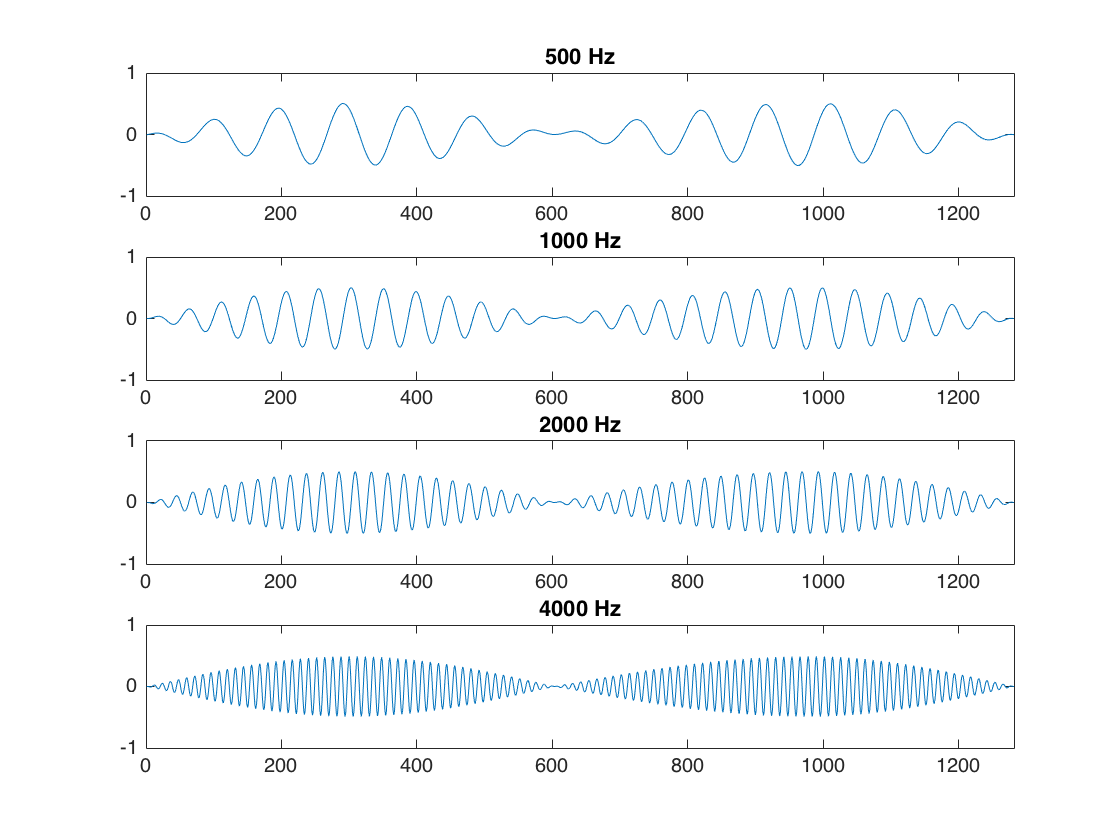
\includegraphics[width=3.5 in]{stimulus}
\caption{Stimulus Centered on Temporal Envelope Shift}
\label{fig:stimulus}
\end{figure}
%%%%%%%%%%%% FIGURE (STIM) %%%%%%%%%%%%
 
Subjects were presented with 4 second long amplitude modulated sine tones with a change in temporal envelope after 2 seconds. Between each tone was 1.5 seconds of silence for a total stimulus onset asynchrony (SOA) of 5.5 seconds. The carrier frequency of these tones were either $500$ Hz, $1000$ Hz, $2000$ Hz, or $4000$ Hz. The amplitude modulation frequency stayed constant at $40$ Hz \textbf{Fig~\ref{fig:stimulus}}. 

%%%%%%%%%%%% FIGURE (AM) %%%%%%%%%%%% 
\begin{figure}[t]
\centering
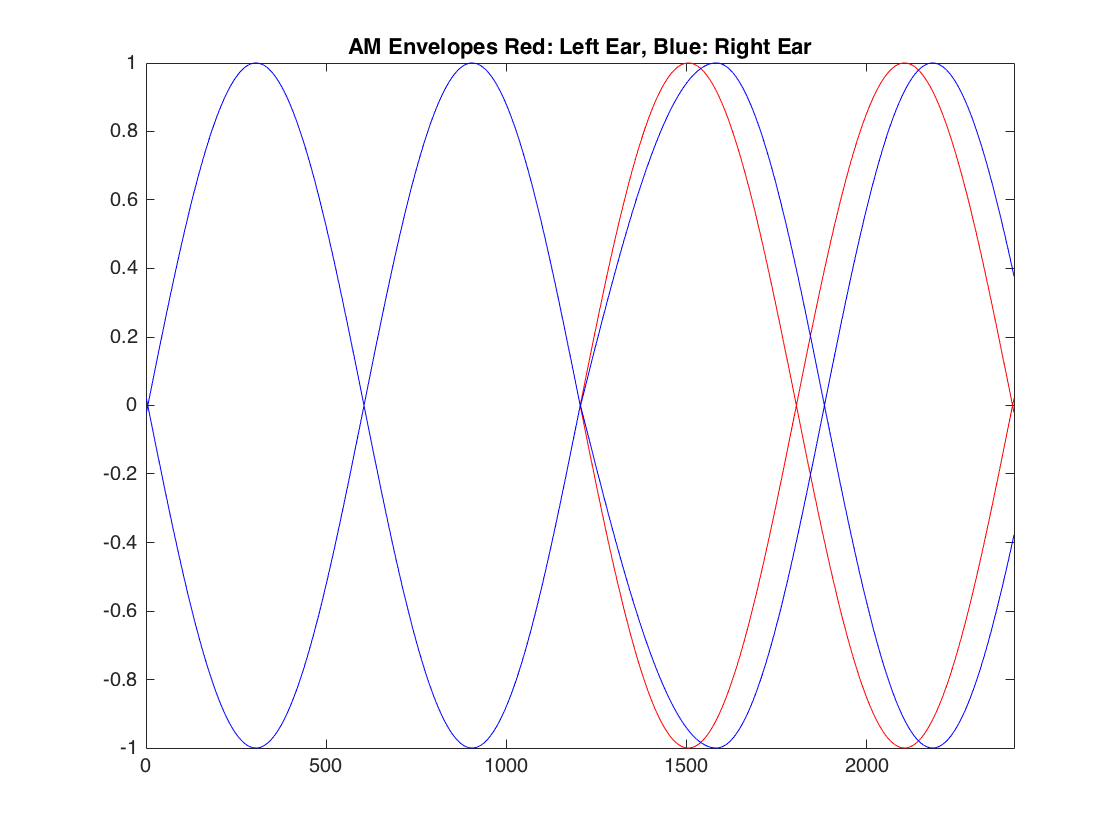
\includegraphics[width=3.5 in]{AM}
\caption{Amplitude Modulation Envelopes}
\label{fig:AM}
\end{figure}
%%%%%%%%%%%% FIGURE (AM) %%%%%%%%%%%%
 
%%%%%%%%%%%% FIGURE (ELC) %%%%%%%%%%%% 
\begin{figure}[b]
\centering
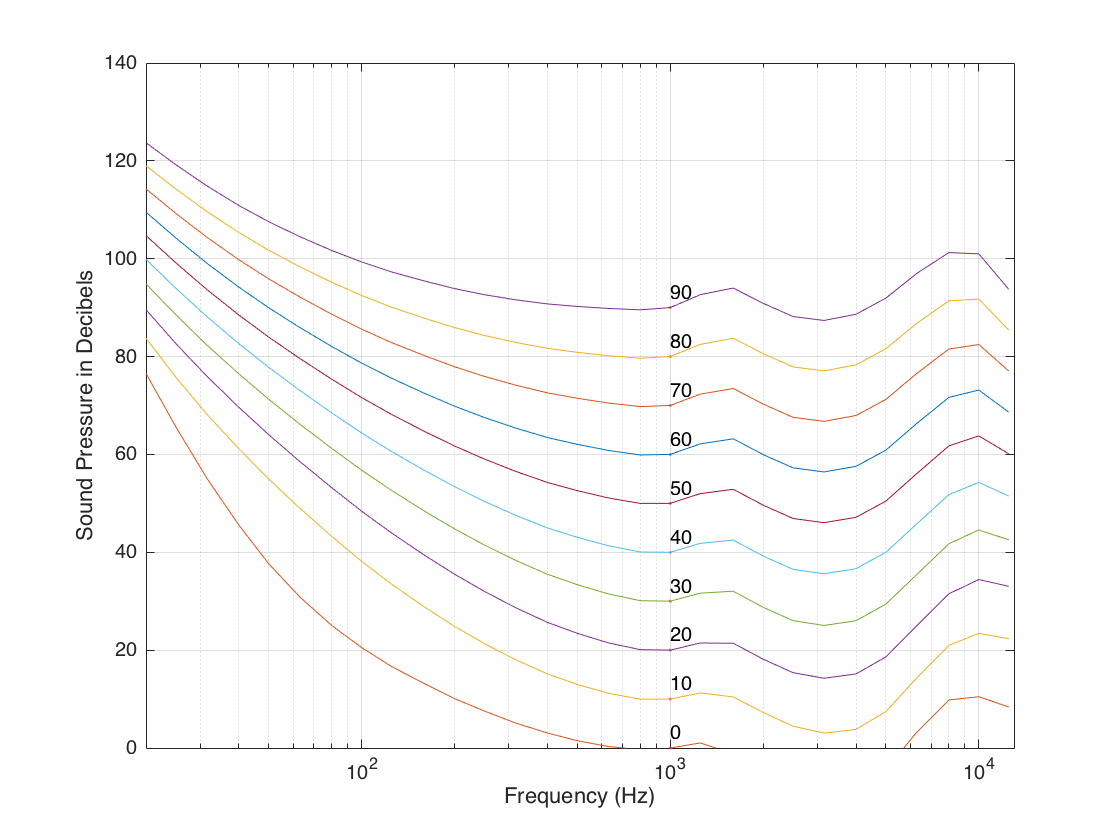
\includegraphics[width=3.5 in]{ELC}
\caption{Equal loudness contours}
\label{fig:ELC}
\end{figure}
%%%%%%%%%%%% FIGURE (ELC) %%%%%%%%%%%%
 
%%%%%%%%%%% FIGURE (erp_chart) %%%%%%%%%%%% 
\begin{figure}[b]
\centering
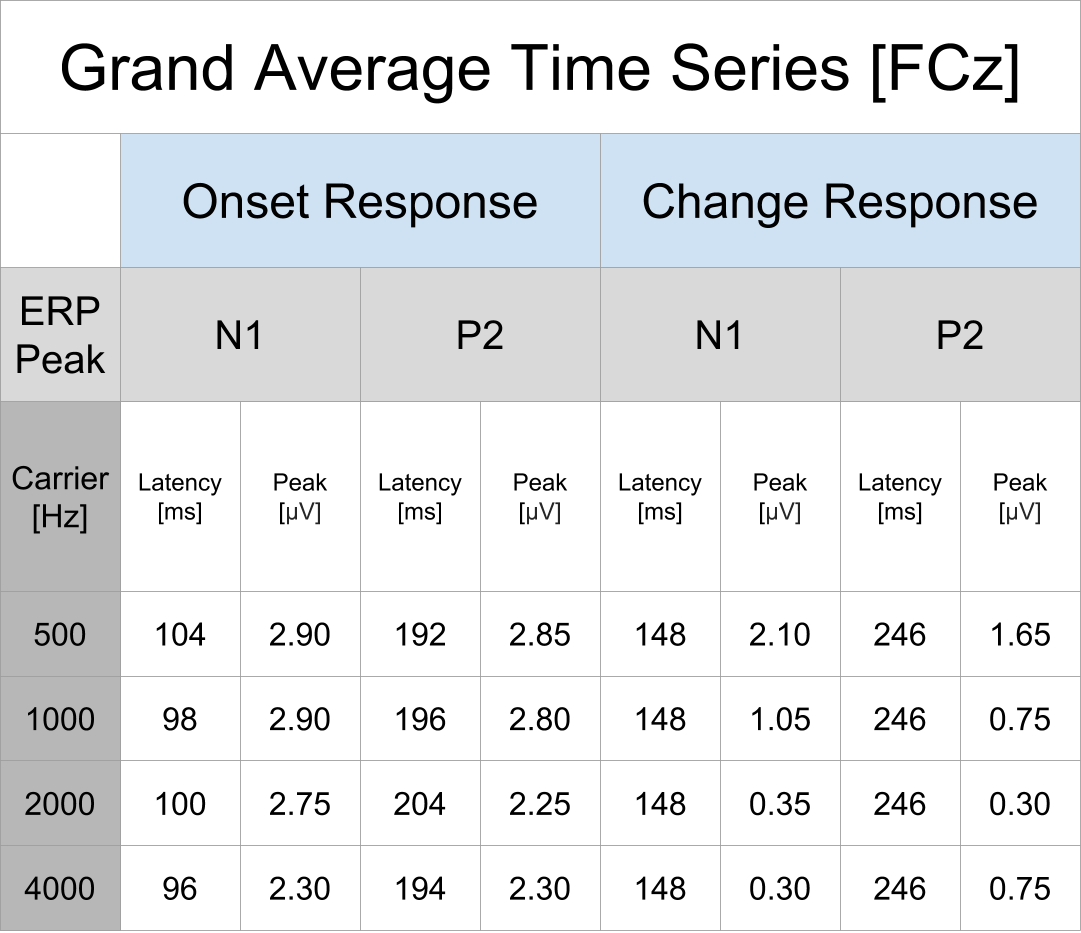
\includegraphics[width=3.0 in]{erp_chart.png}
\caption{N1 and P2 Peaks and Latencies}
\label{fig:erp_chart}
\end{figure}
%%%%%%%%%%% FIGURE (erp_chart) %%%%%%%%%%%%

\subsection{The Stimuli}
For the first 2 seconds of each tone, both ears received the same diotic signal. At 2 seconds, the phase of the temporal envelope in the right ear was shifted by $1.5$ ms, equivalent to a quarter cycle of the $40$ Hz modulation. To smooth this transition, a $1.5$ ms section of a $31.8471$ Hz AM signal was fit to this delay \textbf{Fig~\ref{fig:AM}}. resulting in a temporal envelope difference between the left and right ear inputs. Note that the carrier frequency phase was kept identical between the ears throughout the tone duration. The effect of this was a delay in temporal envelope that was not perceivable when listening only to the signal in the right ear. This created a dichotic signal when heard binaurally, shifting the apparent location of the sound. While the carrier frequency varied by condition, the phase of the carrier signal was always kept identical between the left and right ears. To prevent a discontinuity at the end of the delayed signal, the last $6.25$ ms of both channels were ramped to zero with a cosine curve.
%------------------------------------------------------------------------------------------------------------------
%	FIGURES FIGURES FIGURES FIGURES FIGURES FIGURES FIGURES
%------------------------------------------------------------------------------------------------------------------

%---------------------------------------------------------------------------------------------
%	           OVERLAYS	      OVERLAYS           OVERLAYS
%---------------------------------------------------------------------------------------------
%---------------------------------------------------
%	           GRAND AVERAGE
%---------------------------------------------------

%%%%%%%%%%%% FIGURE (GA_diotic) %%%%%%%%%%%% 
\begin{figure}[t]
\centering
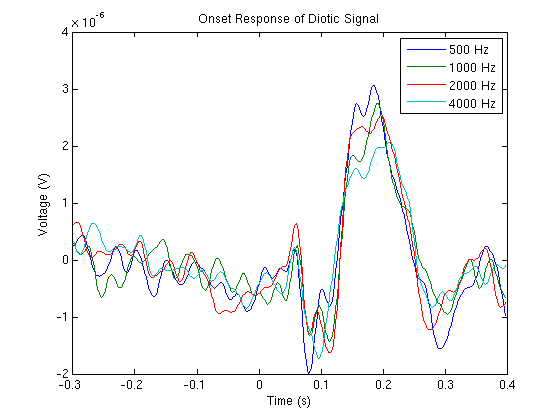
\includegraphics[width=3.5 in]{GA_diotic}
\caption{Grand Average: Onset Response}
\label{fig:GA_diotic}
\end{figure}
%%%%%%%%%%%% FIGURE (GA_diotic) %%%%%%%%%%%%

%%%%%%%%%%% FIGURE (GA_dichotic) %%%%%%%%%%%% 
\begin{figure}[t]
\centering
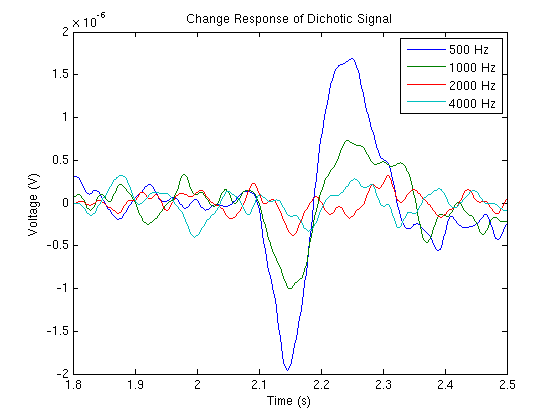
\includegraphics[width=3.5 in]{GA_dichotic}
\caption{Grand Average: Dichotic 500 Hz}
\label{fig:GA_dichotic}
\end{figure}
%%%%%%%%%%% FIGURE (GA_dichotic) %%%%%%%%%%%%

\subsubsection{Equal Loudness Compensation}
In order to control for the apparent loudness of the 4 different carrier frequencies, an equal loudness curve (ELC) was applied to the stimuli.  Although based on perceived loudnesses, the dB[EQL] sound pressure weighting is not a specific loudness measurement, does not consider critical band formation, and does not yield masking or psychoacoustic loudness data\cite{ISO226€2003}. The ELC served as a spectral `weighting' intended to match the sensitivity of hearing as a function of frequency within ``use-level" ranges, specifically accounting for  cavum conchae resonance of the ear.  Sound intensity was set as reference at $80$ Phon for the 1000 Hz carrier frequency prior to amplitude modulation.  Relative amplitudes for all other carrier frequencies were tuned according to their respective ISO 226:2003 standard ELC characteristics \textbf{Fig~\ref{fig:ELC}}.  However, since these stimuli were complex tones, additional calibration was needed. A pilot hearing threshold test was conducted on 2 subjects. Both subjects heard stimuli from all 4 conditions starting at silence until they reported hearing the tone. The results from both subjects were averaged to create an additional volume offset and the averaged hearing threshold using STIM2\cite{STIM} stimulus presentation software.  The final volume offsets were based on a sound intensity of 80 dB-SPL as reference for the 1000 Hz stimulus, resulting in normailzed gains of 87, 75.5, 76 dB-SPL for the 500, 2000 and 4000 Hz stimulus respectively.  

\subsection{Participants}
There were 6 participants in this study (3 male, 3 female) between the ages of 23-31. 5 of the 6 participants had some form of musical training. One participant was left-handed.


\subsection{EEG recording procedure}
Each block consisted of 100 trials in a single condition. Participants each experienced 8 blocks, 2 for each condition. This brought the time for each block to 9 minutes and 10 seconds, and the total time for each subject to 73 minutes and 20 seconds.  Prep time and capping each participant added roughly 30 minutes to each session.\\

During the recording time, participants were seated in a comfortable reclining chair in an electrically shielded room. Participants were presented the movie or show of their choice with subtitles and were instructed to fixate their eyes on the screen and move a little as possible.
%%%%%%%%%%%% FIGURE (BOX N1 Onset Response) %%%%%%%%%%%% 
\begin{figure}[t]
\centering
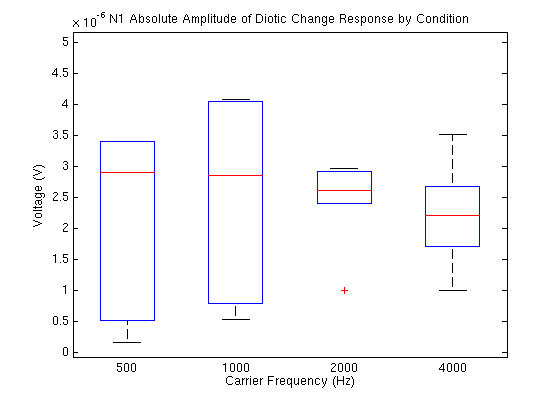
\includegraphics[width=3.5 in]{box_diotic_N1}
\caption{N1 Onset Response}
\label{fig:box_diotic_N1}
\end{figure}
%%%%%%%%%%%% FIGURE (BOX N1 Onset Response) %%%%%%%%%%%%

%%%%%%%%%%%% FIGURE (BOX P2 Onset Response) %%%%%%%%%%%% 
\begin{figure}[t]
\centering
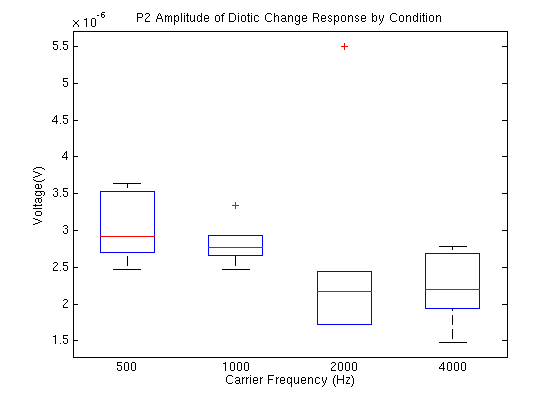
\includegraphics[width=3.5 in]{box_diotic_P2}
\caption{P2 Onset Response}
\label{fig:box_diotic_P2}
\end{figure}
%%%%%%%%%%%% FIGURE (BOX P2 Onset Response) %%%%%%%%%%%%

\subsection{Data analysis}
Before processing the data, a signal space projector (SSP) was created to detect eye blinks using data from electrodes located above and below the left eye and on each temple. This SSP was generated and applied  with the Brainstorm3 Matlab toolbox \cite{Brainstorm} using ocular artifact reduction (OAR)  based on vertical electrooculographic (EEG-VEOG) and horizontal electrooculographic (EEG-HEOG) covariance analysis, derived from EEG measurements taken at the right temple, lower brow, upper check bone, and temple surrounding the left eye of each subject. This SSP was applied to each epoch to remove eye blink artifacts. There was no peak to peak artifact detection performed and all 200 trials from each condition were used to compute single subject and grand averages. The electrode FCz showed very strong onset and change responses, and was chosen to visualize the ERP components in the overlay and box plots.


%%%%%%%%%%%% FIGURE (GA_Change_N1_500) %%%%%%%%%%%% 
\begin{figure}[b]
\centering
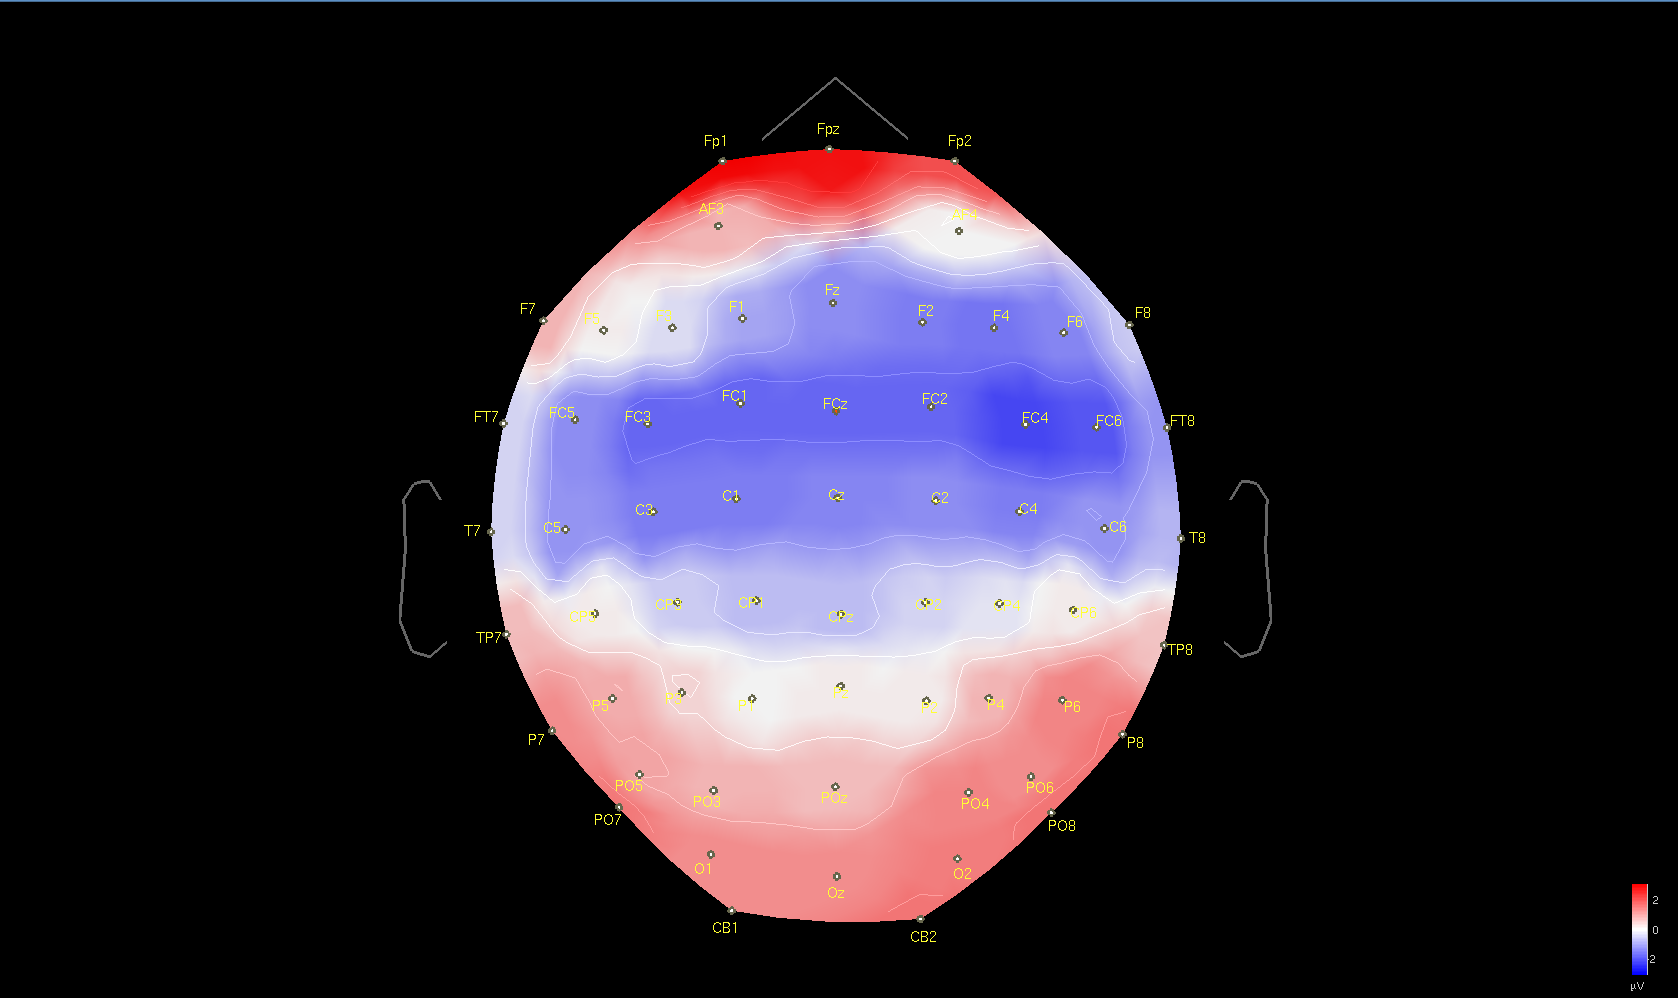
\includegraphics[width=3.0 in]{GA_Change_N1_500}
\caption{Grand Average: Change N1 500 Hz}
\label{fig:GA_Change_N1_500}
\end{figure}
%%%%%%%%%%%% FIGURE (GA_Change_N1_500) %%%%%%%%%%%%

%----------------------------------------------------------------------------------------
%	RESULTS
%----------------------------------------------------------------------------------------

%%%%%%%%%%%% FIGURE (BOX N1 Change Response) %%%%%%%%%%%% 
\begin{figure}[t]
\centering
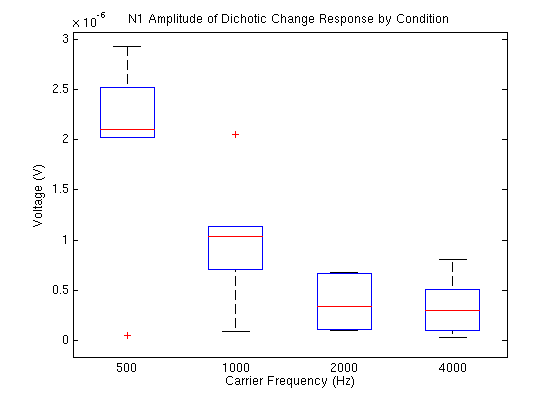
\includegraphics[width=3.5 in]{box_dichotic_N1}
\caption{N1 Change Response}
\label{fig:box_dichotic_N1}
\end{figure}
%%%%%%%%%%%% FIGURE (BOX N1 Change Response) %%%%%%%%%%%%

%%%%%%%%%%%% FIGURE (BOX P2 Change Response) %%%%%%%%%%%% 
\begin{figure}[t]
\centering
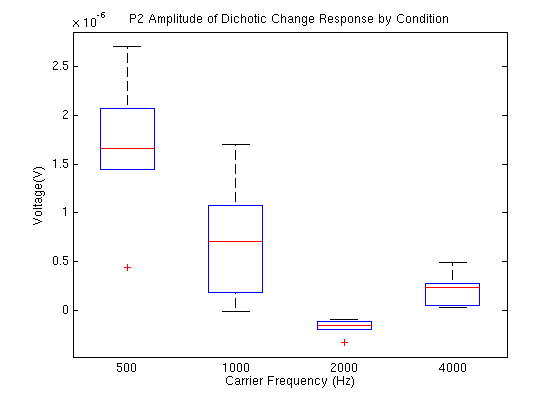
\includegraphics[width=3.5 in]{box_dichotic_P2}
\caption{P2 Change Response}
\label{fig:box_dichotic_P2}
\end{figure}
%%%%%%%%%%%% FIGURE (BOX P2 Change Response) %%%%%%%%%%%%
\section{Results}
The diotic conditions showed no significant changes in peak and latency characteristics across conditions, confirming successful equal loudness calibration across carrier frequencies \textbf{Fig~\ref{fig:GA_diotic}}.   In contrast, a large difference was clearly seen between the 500 Hz stimulus and the 1000 Hz stimulus in the grand average time series waveforms \textbf{Fig~\ref{fig:GA_dichotic}} for the dichotic conditions.  N1 peaks in the grand averged change response were observed at $148$ ms latencies and were observed to be $2.10$ and $1.05$ $\si{\micro} V$  for the $500$ and $1000$ Hz stimulus respectively. The P2 peaks were observed at $246$ ms latencies and were seen to be $1.65$ and $0.75$ $\si{\micro} V$  for the $500$ and $1000$ Hz stimulus respectively \textbf{Fig~\ref{fig:erp_chart}}\textbf{,~\ref{fig:GA_dichotic}}. Without further data collection and statistical analysis not much can be said about the difference in the 2000 Hz and 4000 Hz carrier frequencies ERPs.  The responses at these these frequencies were significantly weaker, largely due to greater statistical variance between subjects \textbf{Fig~\ref{fig:erp_chart}}\textbf{,~\ref{fig:GA_dichotic}}.  These results were confirmed by the topographic maps, which showed theses results with both the onset and change response being similarly front central localized \textbf{Fig~\ref{fig:GA_Change_N1_500}}.   Another view of this data and the underlying distribution across subjects can be seen in the box plots for the N1 and P2 peaks in both the onset and change responses \textbf{Fig~\ref{fig:box_diotic_N1}}\textbf{,~\ref{fig:box_diotic_P2}}\textbf{,~\ref{fig:box_dichotic_N1}}\textbf{,~\ref{fig:box_dichotic_P2}}.  All time series plots for each individual participant, as well as topographic maps for the grand average  can be seen in the attached \textbf{appendix}. 
%----------------------------------------------------------------------------------------
%	DISCUSSION
%----------------------------------------------------------------------------------------

\section{Discussion}
While there is not enough data to determine statistical significance, these initial findings show that the response to a dichotic change in temporal envelope does decrease as the carrier frequency increases. However, above 2000 Hz this relationship was not consistent. The difference between the 500 Hz condition and the 1000 Hz condition and between the 1000 Hz condition and the 2000 Hz condition are quite obvious.  A small change response may be present in both of these conditions, which could be an important finding. A difference in the detection threshold frequency between IPD shifts and temporal envelope shifts would suggest that the two features are being processed differently in the brain. \\

It seems logical that the threshold of temporal envelope detection would not be exactly related to the size of a quarter cycle of the carrier frequency, since the carrier frequency phase does not change over the course of the stimuli. However, the reasons for this behavior as a function of carrier frequency is unclear.  There are several aspects of this study that could be improved in future revisions. First, the carrier frequencies chosen did not include those closest to the threshold found by Ross et al \cite{Ross2007}. Adding frequencies near 1250 Hz could help to discern if the threshold for detection of temporal envelope difference differs from the threshold for IPD in carrier frequency. The drawbacks to adding more conditions like this would be the risk of fatiguing participants to the point where their data is no longer reliable.\\

Another future consideration will be to add both behavioral and psychoacoustic components to the study. It is ambiguous whether a change response is present in the 2 highest pitched conditions, but a difference may still have been perceived by the participants. Forming questions similar to Ross et al, future revisions could ask participants if they heard the sound move or if there was any apparent change in timbre. With more research, more participants, and improved control, this study has the potential to further the understanding the effect of complex audio features on sound localization.

	
%----------------------------------------------------------------------------------------
%	BIBLIOGRAPHY
%----------------------------------------------------------------------------------------

\bibliographystyle{apalike} 
\bibliography{ref}


%----------------------------------------------------------------------------------------
%	APPENDIX
%----------------------------------------------------------------------------------------

\clearpage

%\section{Appendix}
%------------------------------------------------------------------------------------------------------------------
%	FIGURES FIGURES FIGURES FIGURES FIGURES FIGURES FIGURES
%------------------------------------------------------------------------------------------------------------------

%---------------------------------------------------------------------------------------------
%	           OVERLAYS	      OVERLAYS           OVERLAYS
%---------------------------------------------------------------------------------------------

%---------------------------------------------------
%	                 SUBJECTS
%---------------------------------------------------

%--------------------------------------
%	                  AL
%--------------------------------------
%%%%%%%%%%%% FIGURE (AL_diotic) %%%%%%%%%%%% 
%\begin{figure}[b]
%\centering
%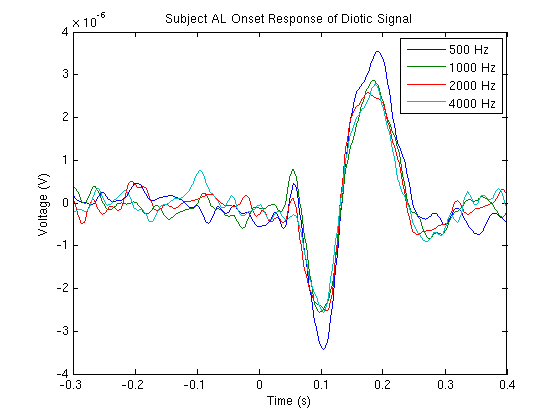
\includegraphics[width=3.5 in]{AL_diotic}
%\caption{Subject 1: Diotic 500 Hz}
%\label{fig:AL_diotic}
%\end{figure}
%%%%%%%%%%%% FIGURE (AL_diotic) %%%%%%%%%%%%
%
%%%%%%%%%%%% FIGURE (AL_dichotic) %%%%%%%%%%%% 
%\begin{figure}[b]
%\centering
%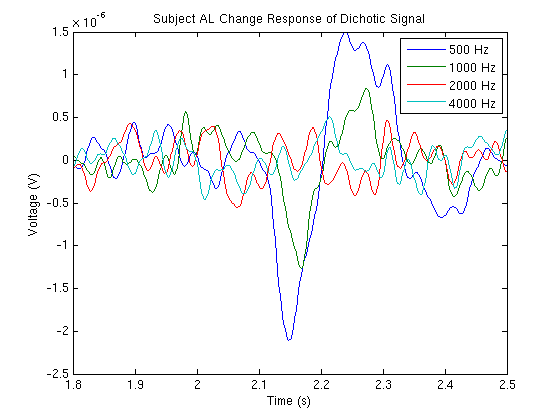
\includegraphics[width=3.5 in]{AL_dichotic}
%\caption{Subject 1: Dichotic 500 Hz}
%\label{fig:AL_dichotic}
%\end{figure}
%%%%%%%%%%%% FIGURE (AL_dichotic) %%%%%%%%%%%%
%--------------------------------------
%	                 CM
%--------------------------------------
%%%%%%%%%%%% FIGURE (CM_diotic) %%%%%%%%%%%% 
%\begin{figure}[b]
%\centering
%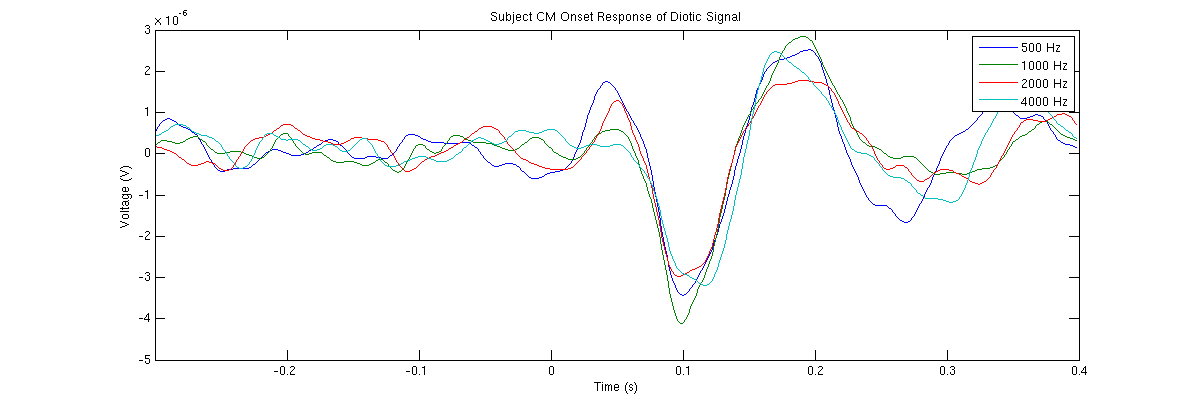
\includegraphics[width=3.5 in]{CM_diotic}
%\caption{Subject 2: Diotic 500 Hz}
%\label{fig:CM_diotic}
%\end{figure}
%%%%%%%%%%%% FIGURE (CM_diotic) %%%%%%%%%%%%
%
%%%%%%%%%%%% FIGURE (CM_dichotic) %%%%%%%%%%%% 
%\begin{figure}[b]
%\centering
%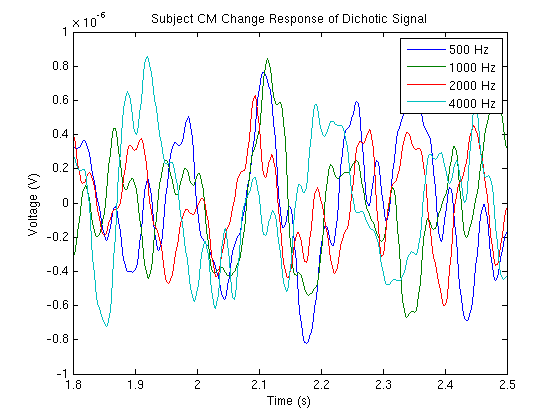
\includegraphics[width=3.5 in]{CM_dichotic}
%\caption{Subject 2: Dichotic 500 Hz}
%\label{fig:CM_dichotic}
%\end{figure}
%%%%%%%%%%%% FIGURE (CM_dichotic) %%%%%%%%%%%%
%
%\clearpage
%
%--------------------------------------
%	                 MH
%--------------------------------------
%%%%%%%%%%%% FIGURE (MH_diotic) %%%%%%%%%%%% 
%\begin{figure}[b]
%\centering
%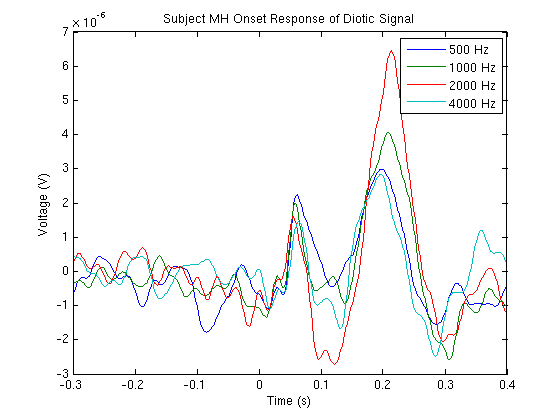
\includegraphics[width=3.5 in]{MH_diotic}
%\caption{Subject 3: Diotic 500 Hz}
%\label{fig:MH_diotic}
%\end{figure}
%%%%%%%%%%%% FIGURE (MH_diotic) %%%%%%%%%%%%
%
%%%%%%%%%%%% FIGURE (MH_dichotic) %%%%%%%%%%%% 
%\begin{figure}[b]
%\centering
%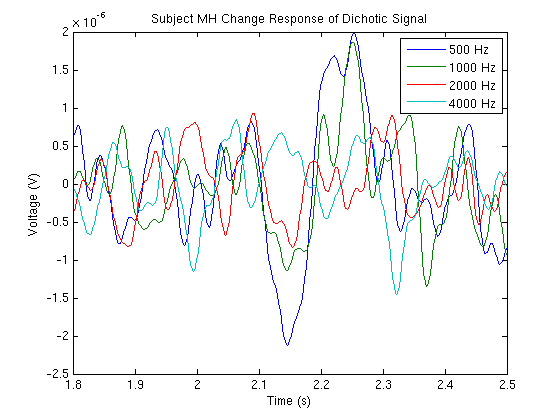
\includegraphics[width=3.5 in]{MH_dichotic}
%\caption{Subject 3: Dichotic 500 Hz}
%\label{fig:MH_dichotic}
%\end{figure}
%%%%%%%%%%%% FIGURE (MH_dichotic) %%%%%%%%%%%%
%--------------------------------------
%	                 NG
%--------------------------------------
%
%%%%%%%%%%%% FIGURE (NG_diotic) %%%%%%%%%%%% 
%\begin{figure}[b]
%\centering
%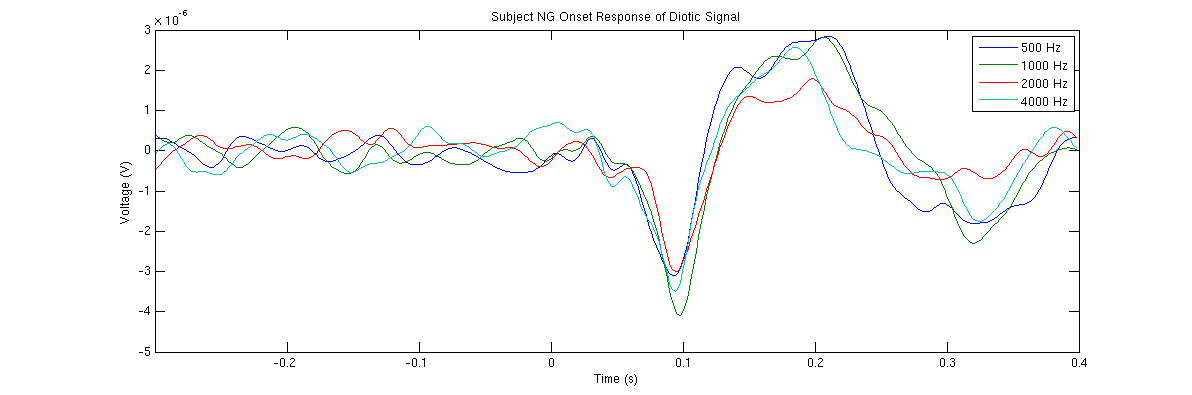
\includegraphics[width=3.5 in]{NG_diotic}
%\caption{Subject 4: Diotic 500 Hz}
%\label{fig:NG_diotic}
%\end{figure}
%%%%%%%%%%%% FIGURE (NG_diotic) %%%%%%%%%%%%
%
%%%%%%%%%%%% FIGURE (NG_dichotic) %%%%%%%%%%%% 
%\begin{figure}[b]
%\centering
%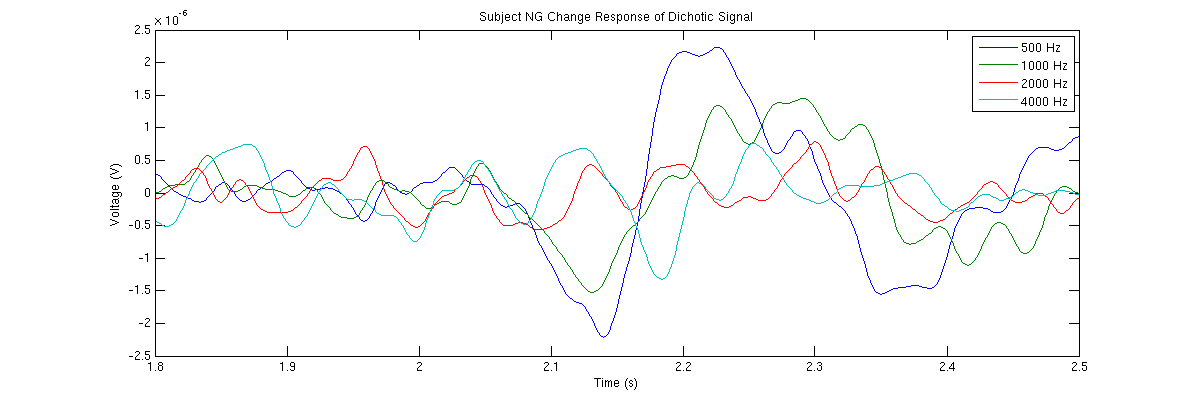
\includegraphics[width=3.5 in]{NG_dichotic}
%\caption{Subject 4: Dichotic 500 Hz}
%\label{fig:NG_dichotic}
%\end{figure}
%%%%%%%%%%%% FIGURE (NG_dichotic) %%%%%%%%%%%%
%
%\clearpage
%
%--------------------------------------
%	                 TD
%--------------------------------------
%%%%%%%%%%%% FIGURE (TD_diotic) %%%%%%%%%%%% 
%\begin{figure}[b]
%\centering
%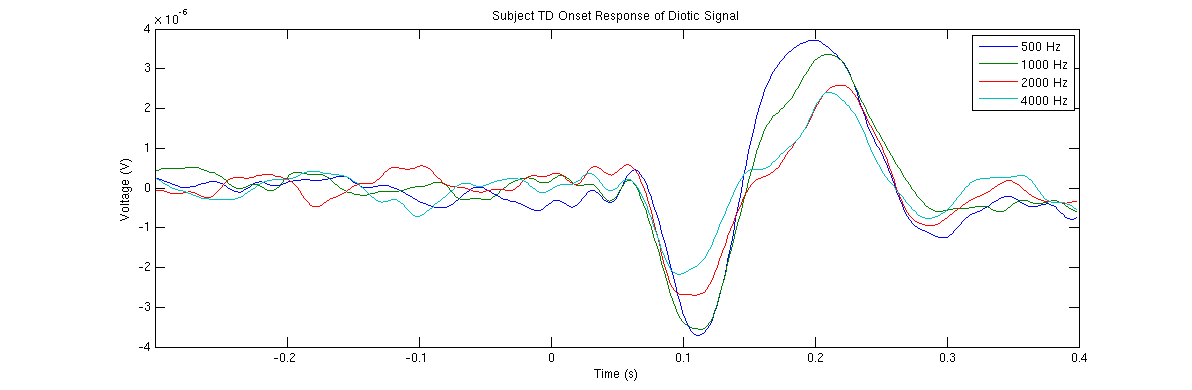
\includegraphics[width=3.5 in]{TD_diotic}
%\caption{Subject 5: Diotic 500 Hz}
%\label{fig:TD_diotic}
%\end{figure}
%%%%%%%%%%%% FIGURE (TD_diotic) %%%%%%%%%%%%
%
%%%%%%%%%%%% FIGURE (TD_dichotic) %%%%%%%%%%%% 
%\begin{figure}[b]
%\centering
%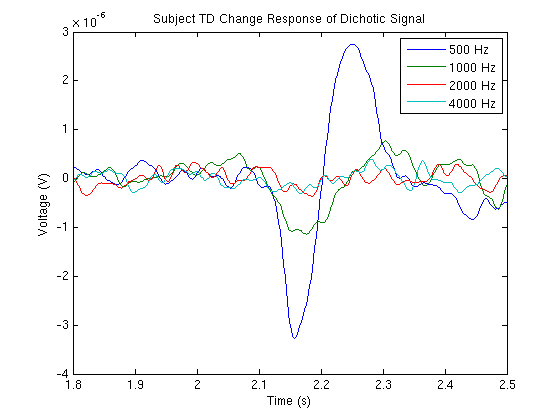
\includegraphics[width=3.5 in]{TD_dichotic}
%\caption{Subject 5: Dichotic 500 Hz}
%\label{fig:TD_dichotic}
%\end{figure}
%%%%%%%%%%%% FIGURE (TD_dichotic) %%%%%%%%%%%%
%--------------------------------------
%	                 WR
%--------------------------------------
%%%%%%%%%%%% FIGURE (WR_diotic) %%%%%%%%%%%% 
%\begin{figure}[b]
%\centering
%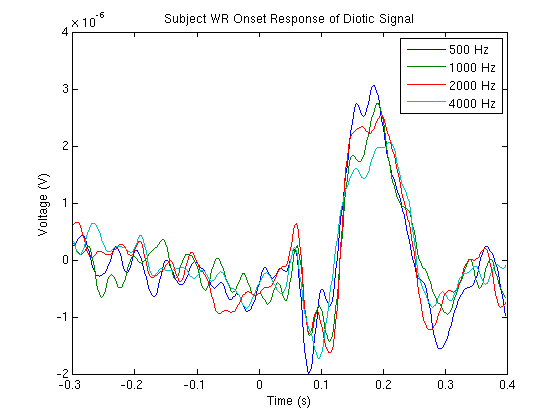
\includegraphics[width=3.5 in]{WR_diotic}
%\caption{Subject 6: Diotic 500 Hz}
%\label{fig:WR_diotic}
%\end{figure}
%%%%%%%%%%%% FIGURE (WR_diotic) %%%%%%%%%%%%
%
%%%%%%%%%%%% FIGURE (WR_dichotic) %%%%%%%%%%%% 
%\begin{figure}[b]
%\centering
%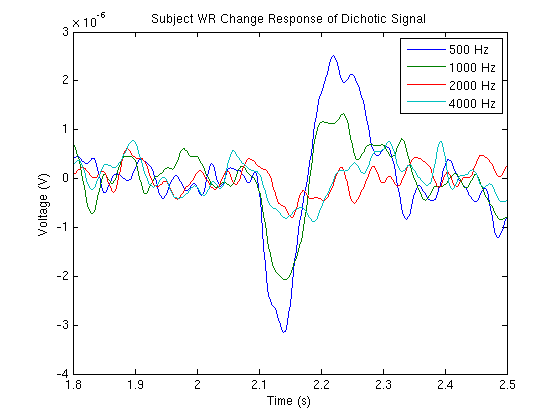
\includegraphics[width=3.5 in]{WR_dichotic}
%\caption{Subject 6: Dichotic 500 Hz}
%\label{fig:WR_dichotic}
%\end{figure}
%%%%%%%%%%%% FIGURE (WR_dichotic) %%%%%%%%%%%%
%
%\clearpage
%
%---------------------------------------------------------------------------------------------
%	         TOPO	      TOPO           TOPO           TOPO       TOPO
%---------------------------------------------------------------------------------------------
%
%---------------------------------------------------------------------------------------------
%	           ONSET RESPONSE	           ONSET RESPONSE
%---------------------------------------------------------------------------------------------
%--------------------------------------
%	           ONSET N1
%--------------------------------------
%
%%%%%%%%%%%% FIGURE (GA_Onset_N1_500) %%%%%%%%%%%% 
%\begin{figure}[b]
%\centering
%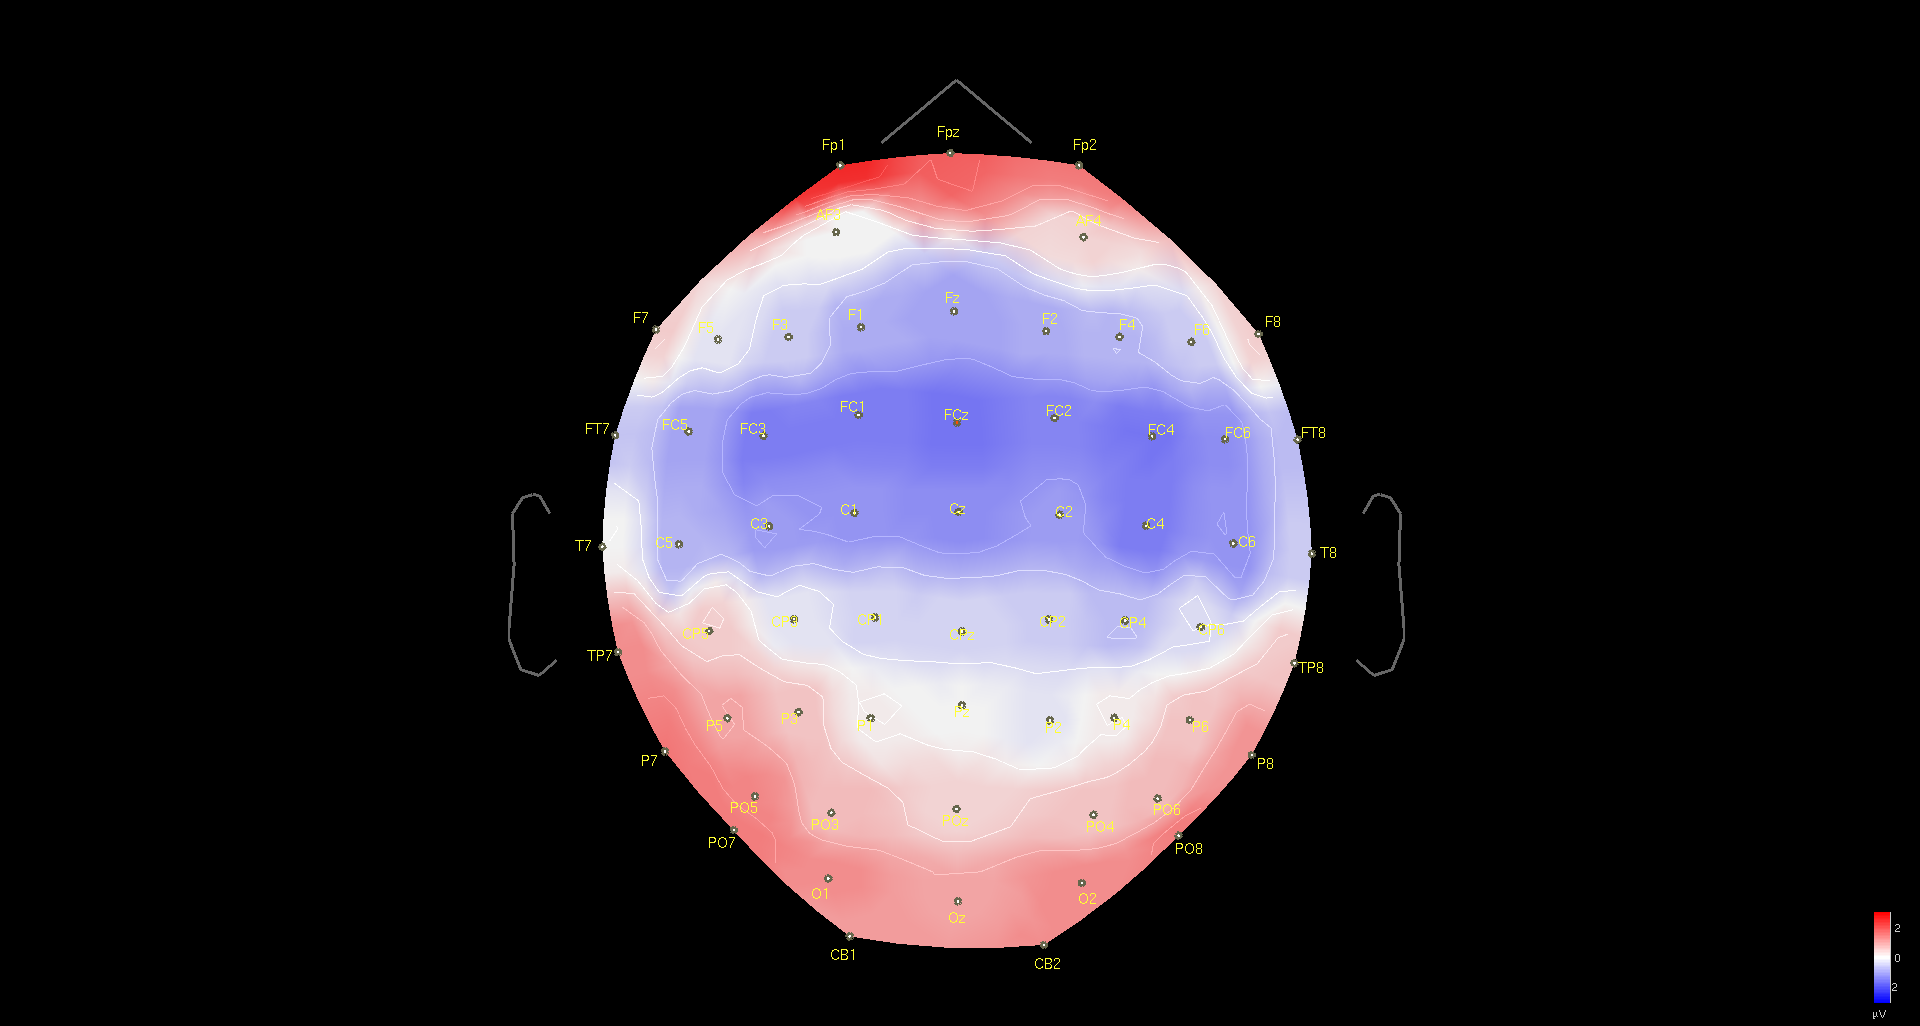
\includegraphics[width=3.5 in]{GA_Onset_N1_500}
%\caption{Grand Average: Onset N1 500 Hz}
%\label{fig:GA_Change_N1_500}
%\end{figure}
%%%%%%%%%%%% FIGURE (GA_Onset_N1_500) %%%%%%%%%%%%
%
%%%%%%%%%%%% FIGURE (GA_Onset_N1_1000) %%%%%%%%%%%% 
%\begin{figure}[b]
%\centering
%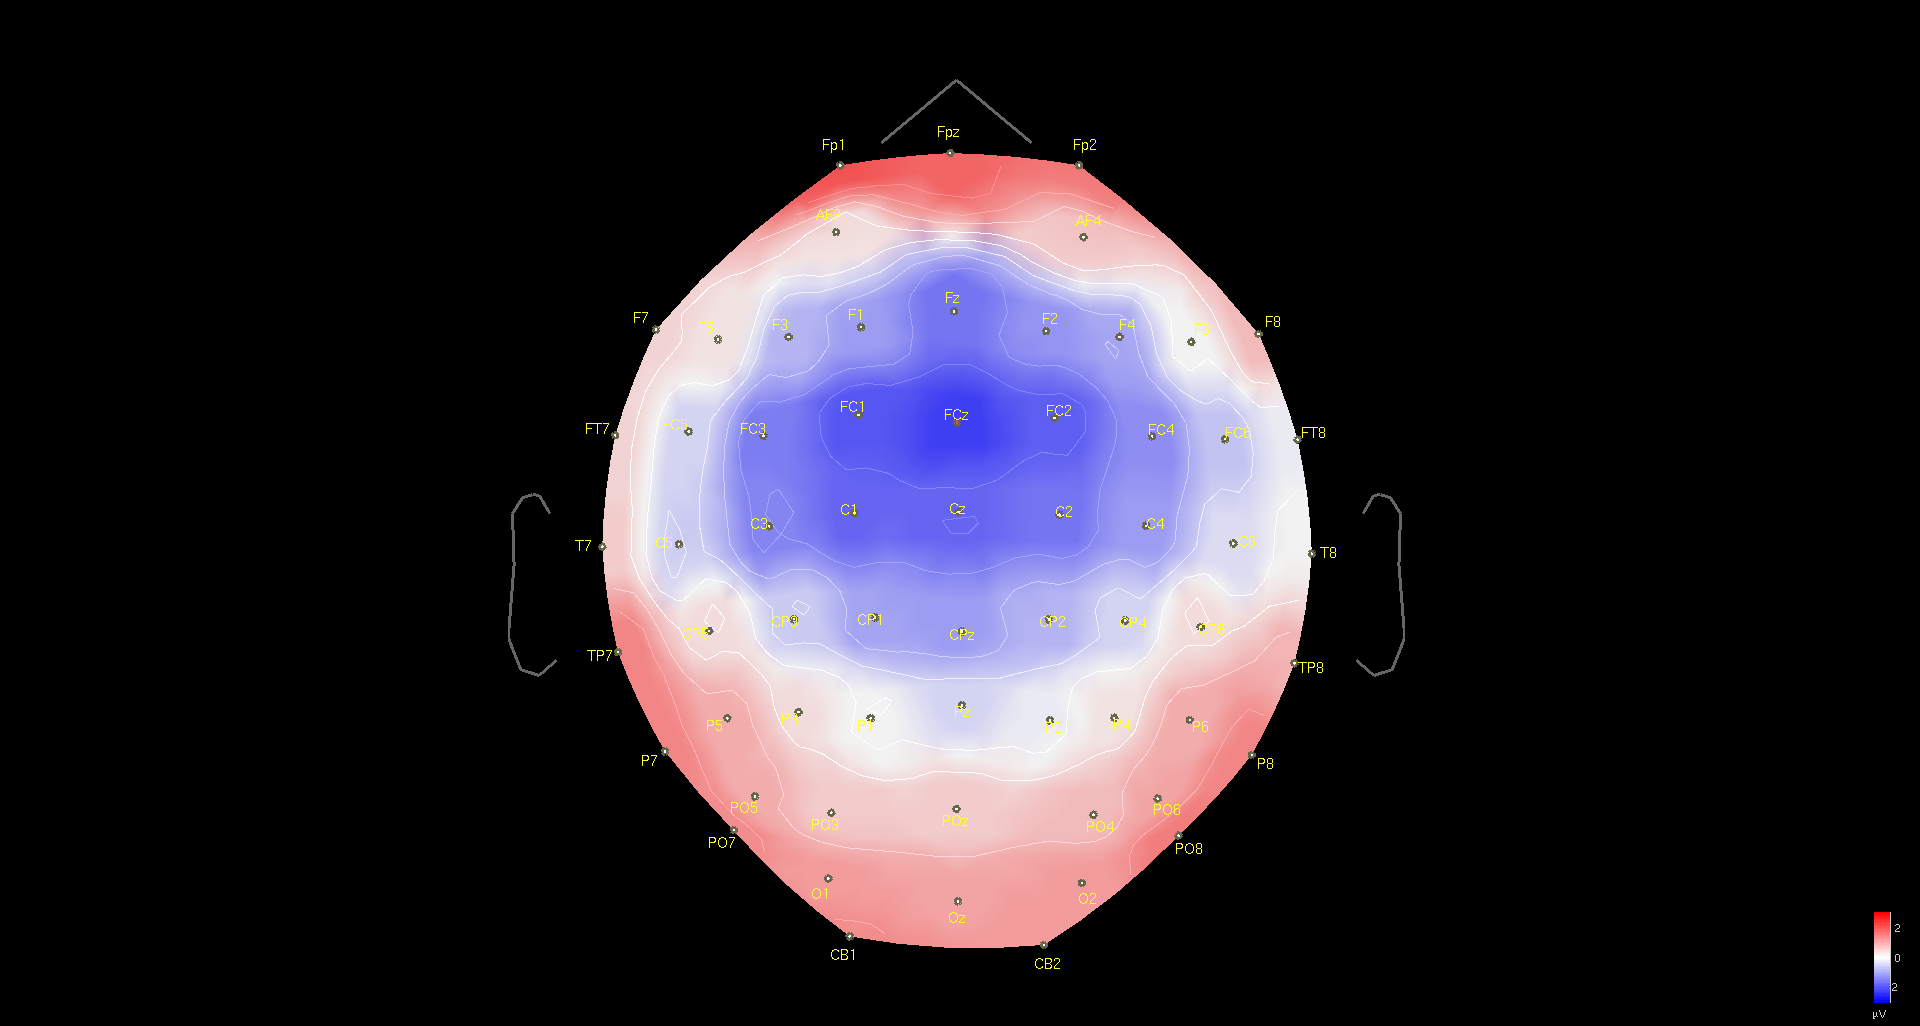
\includegraphics[width=3.5 in]{GA_Onset_N1_1000}
%\caption{Grand Average: Onset N1 1000 Hz}
%\label{fig:GA_Onset_N1_1000}
%\end{figure}
%%%%%%%%%%%% FIGURE (GA_Onset_N1_1000) %%%%%%%%%%%%
%
%%%%%%%%%%%% FIGURE (GA_Onset_N1_2000) %%%%%%%%%%%% 
%\begin{figure}[b]
%\centering
%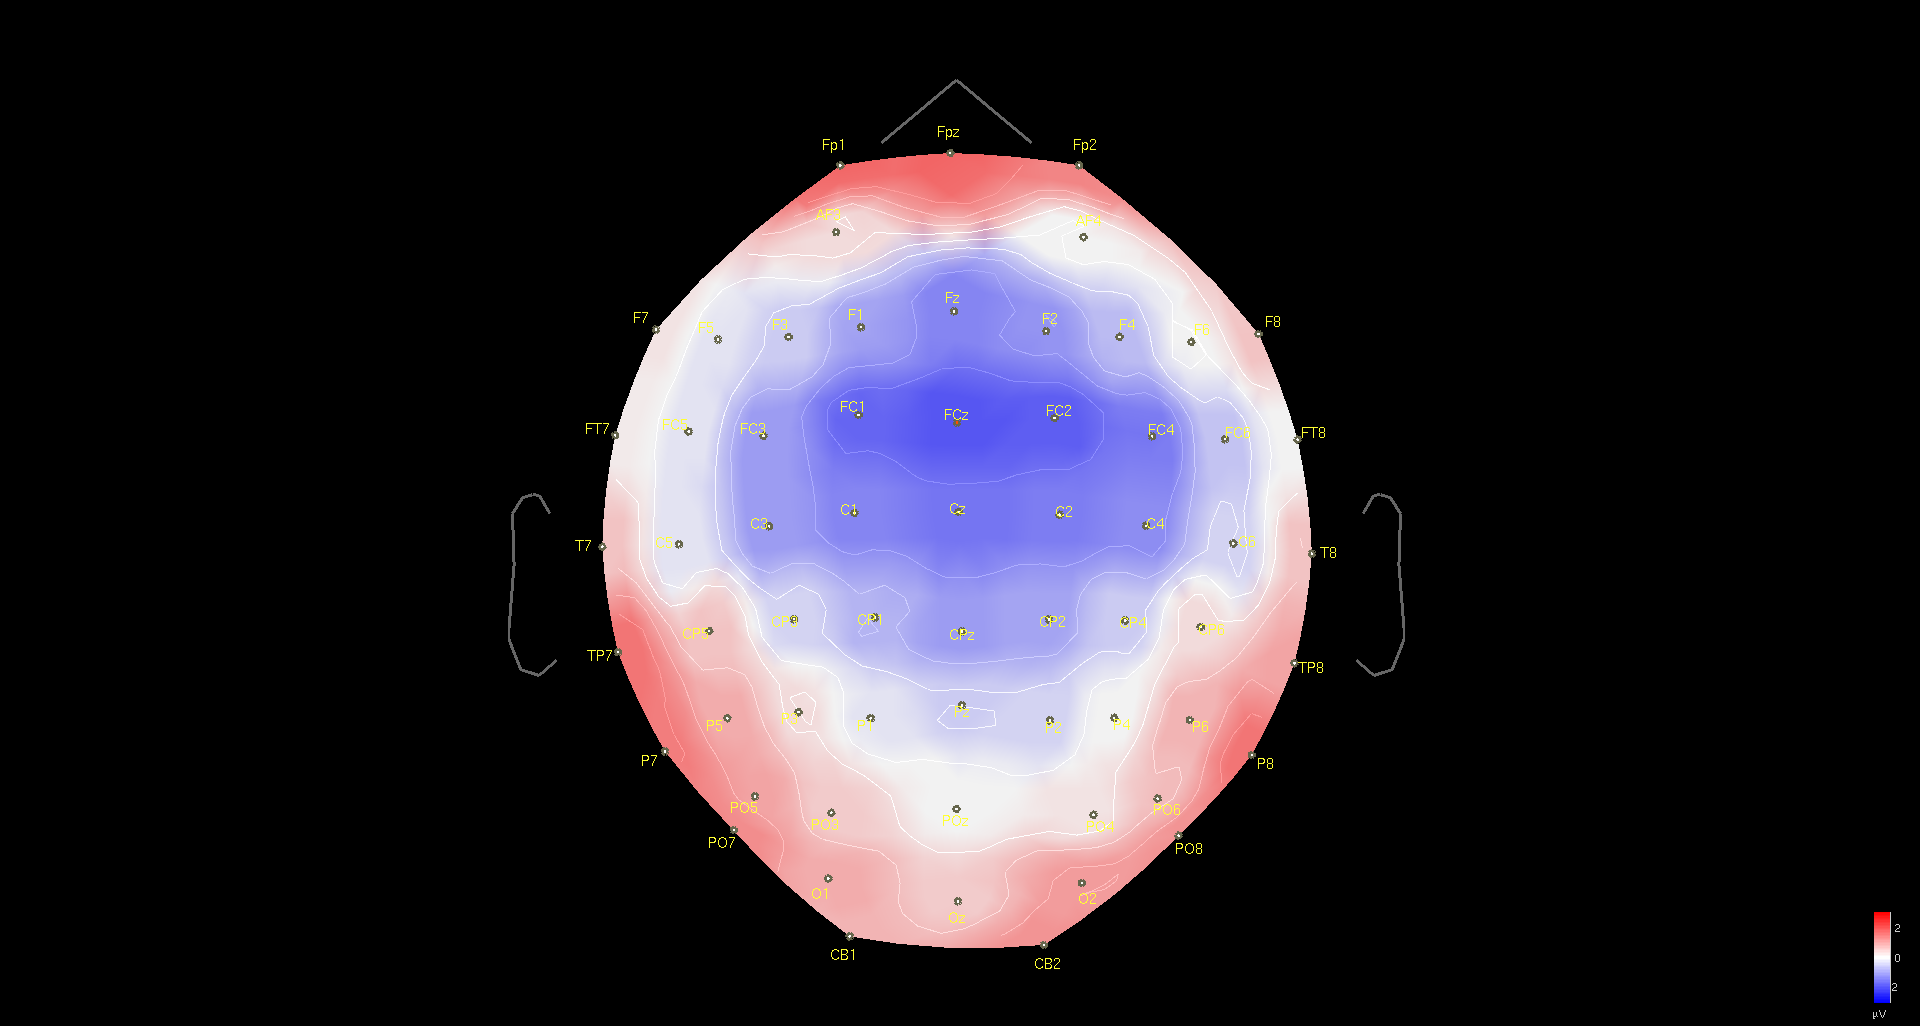
\includegraphics[width=3.5 in]{GA_Onset_N1_2000}
%\caption{Grand Average: Onset N1 2000 Hz}
%\label{fig:GA_Onset_N1_2000}
%\end{figure}
%%%%%%%%%%%% FIGURE (GA_Onset_N1_2000) %%%%%%%%%%%%
%
%%%%%%%%%%%% FIGURE (GA_Onset_N1_4000) %%%%%%%%%%%% 
%\begin{figure}[b]
%\centering
%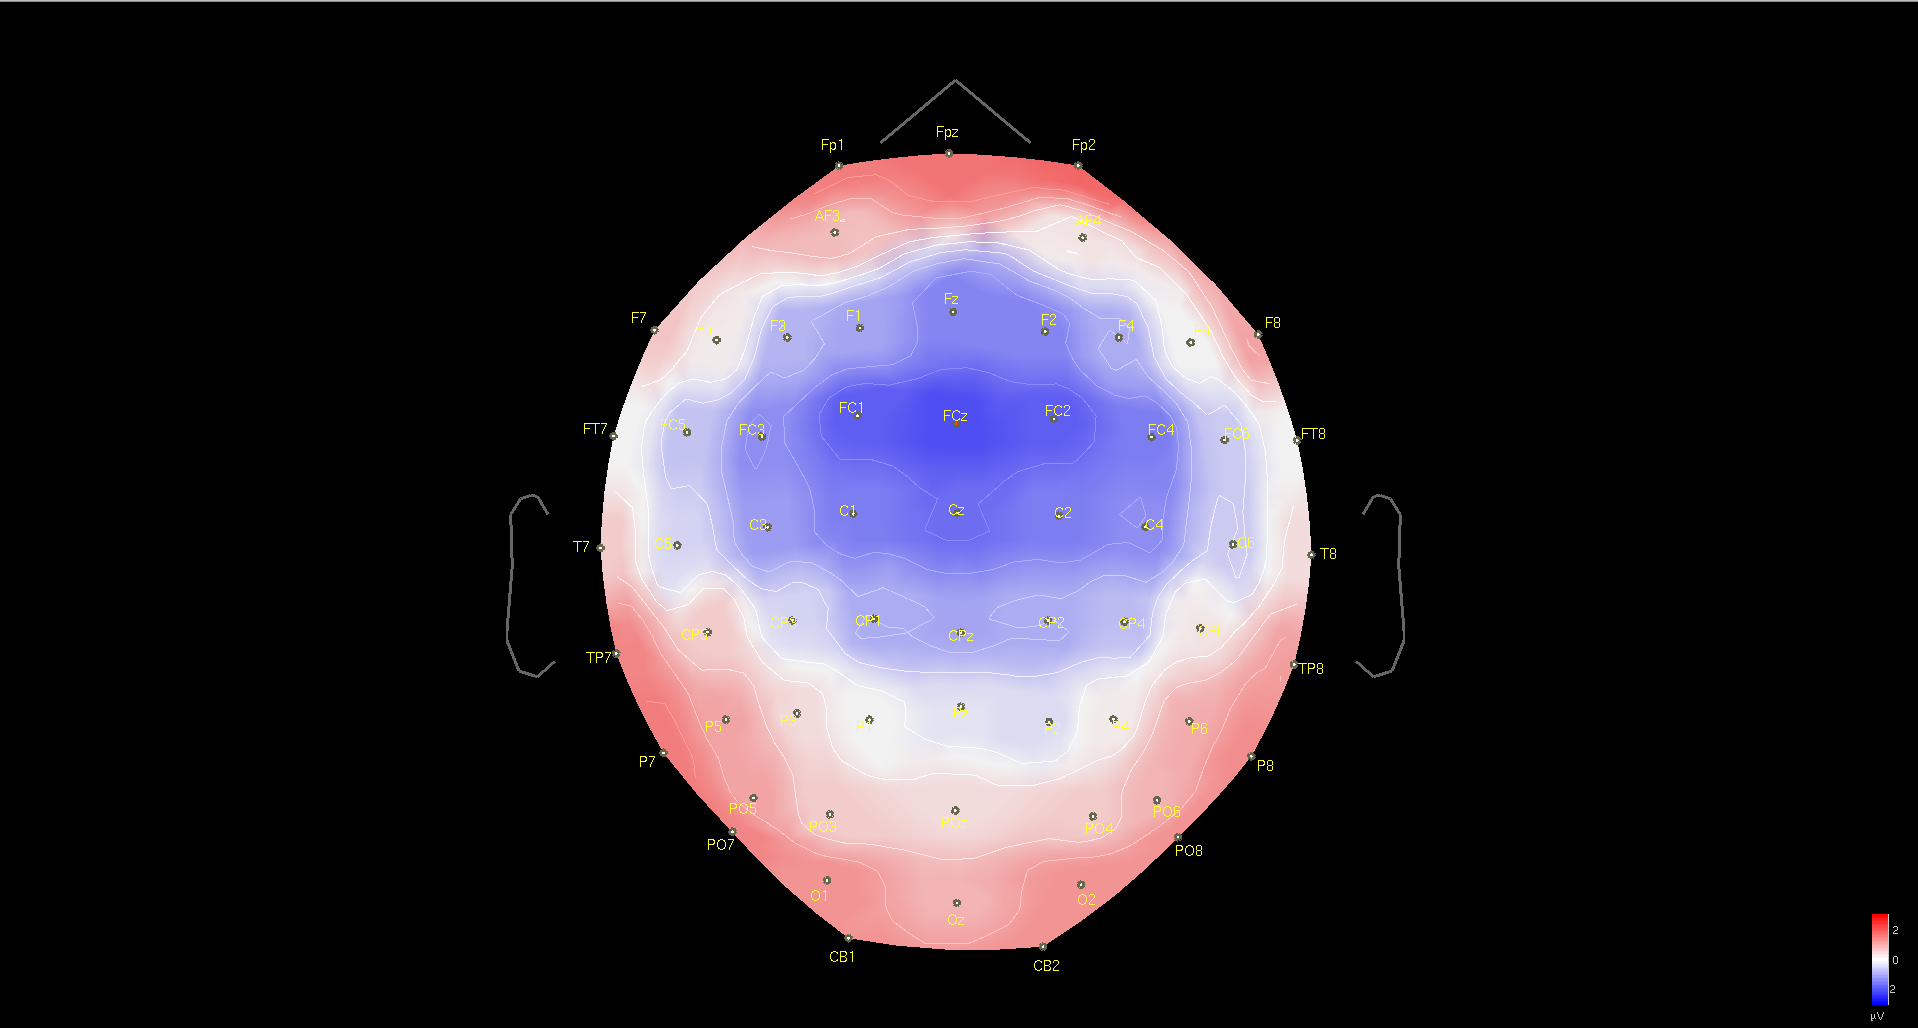
\includegraphics[width=3.5 in]{GA_Onset_N1_4000}
%\caption{Grand Average: Onset N1 4000 Hz}
%\label{fig:GA_Onset_N1_4000}
%\end{figure}
%%%%%%%%%%%% FIGURE (GA_Onset_N1_4000) %%%%%%%%%%%%
%
%--------------------------------------
%	           ONSET P2
%--------------------------------------
%
%%%%%%%%%%%% FIGURE (GA_Onset_P2_500) %%%%%%%%%%%% 
%\begin{figure}[b]
%\centering
%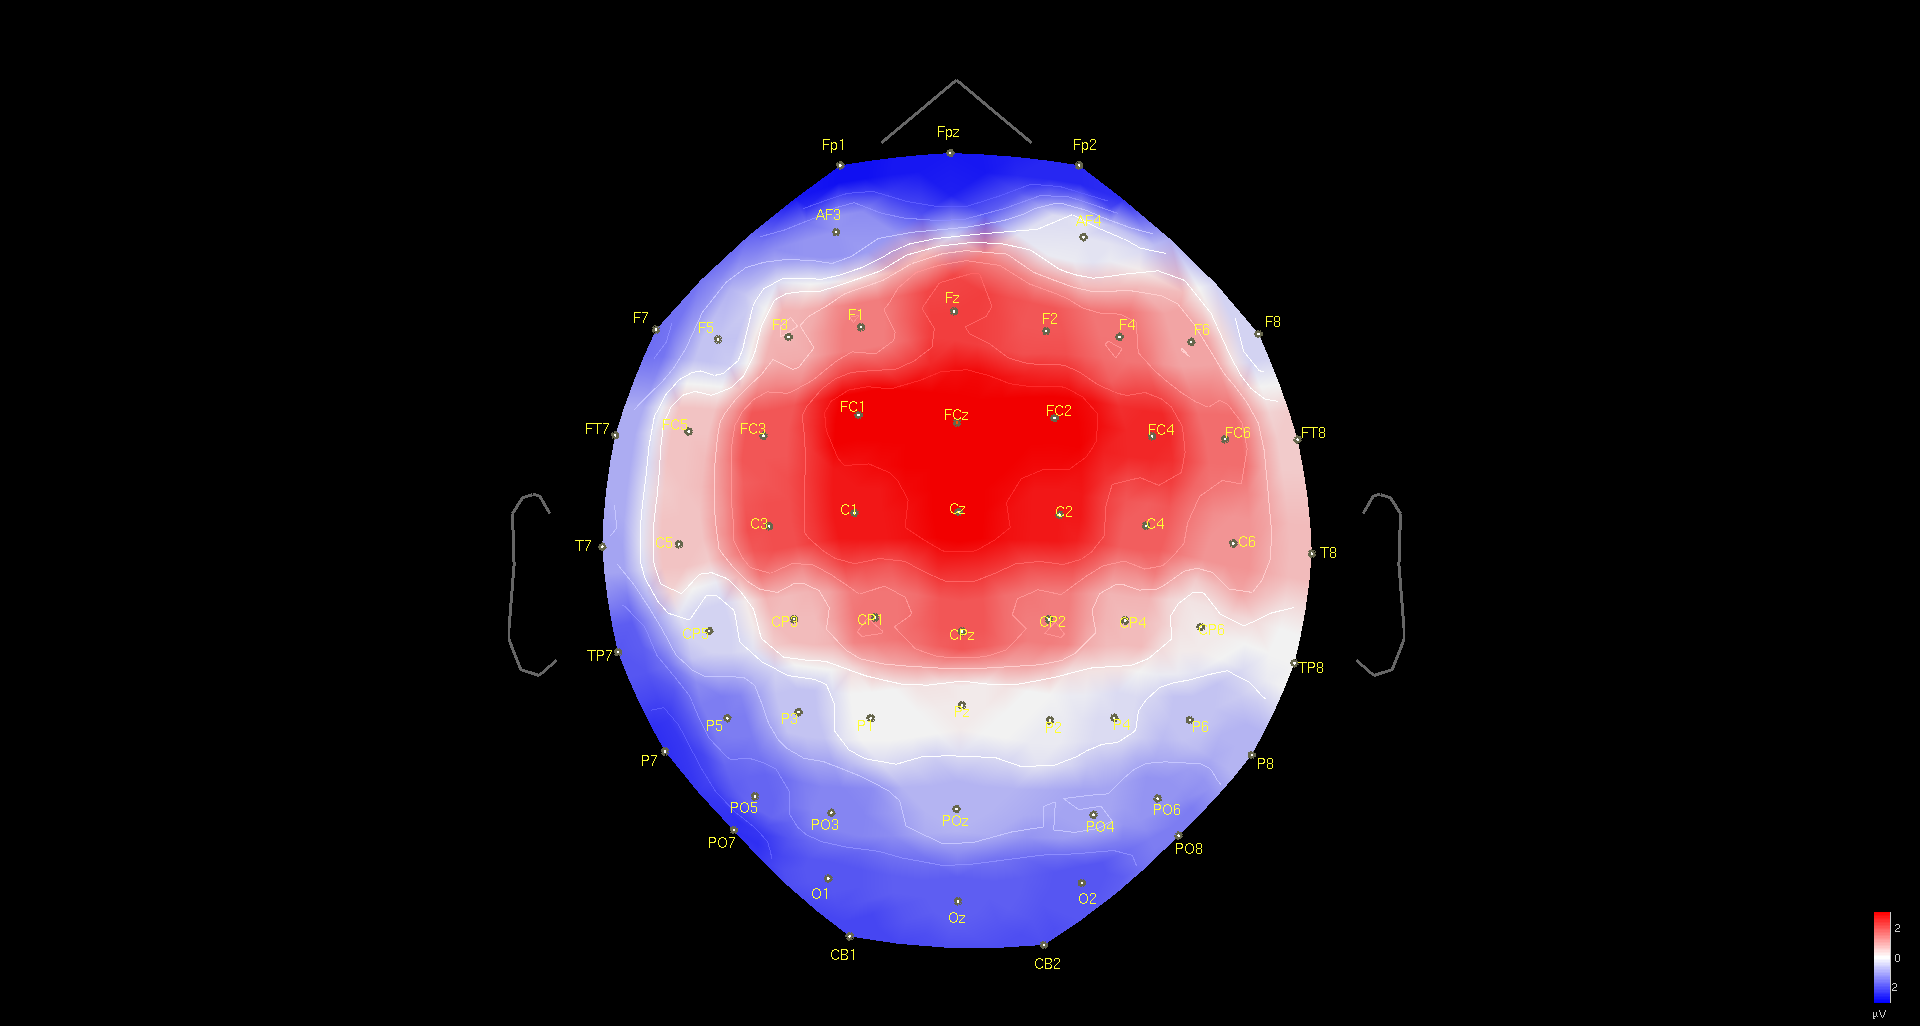
\includegraphics[width=3.5 in]{GA_Onset_P2_500}
%\caption{Grand Average: Onset P2 500 Hz}
%\label{fig:GA_Onset_P2_500}
%\end{figure}
%%%%%%%%%%%% FIGURE (GA_Onset_P2_500) %%%%%%%%%%%%
%
%%%%%%%%%%%% FIGURE (GA_Onset_P2_1000) %%%%%%%%%%%% 
%\begin{figure}[b]
%\centering
%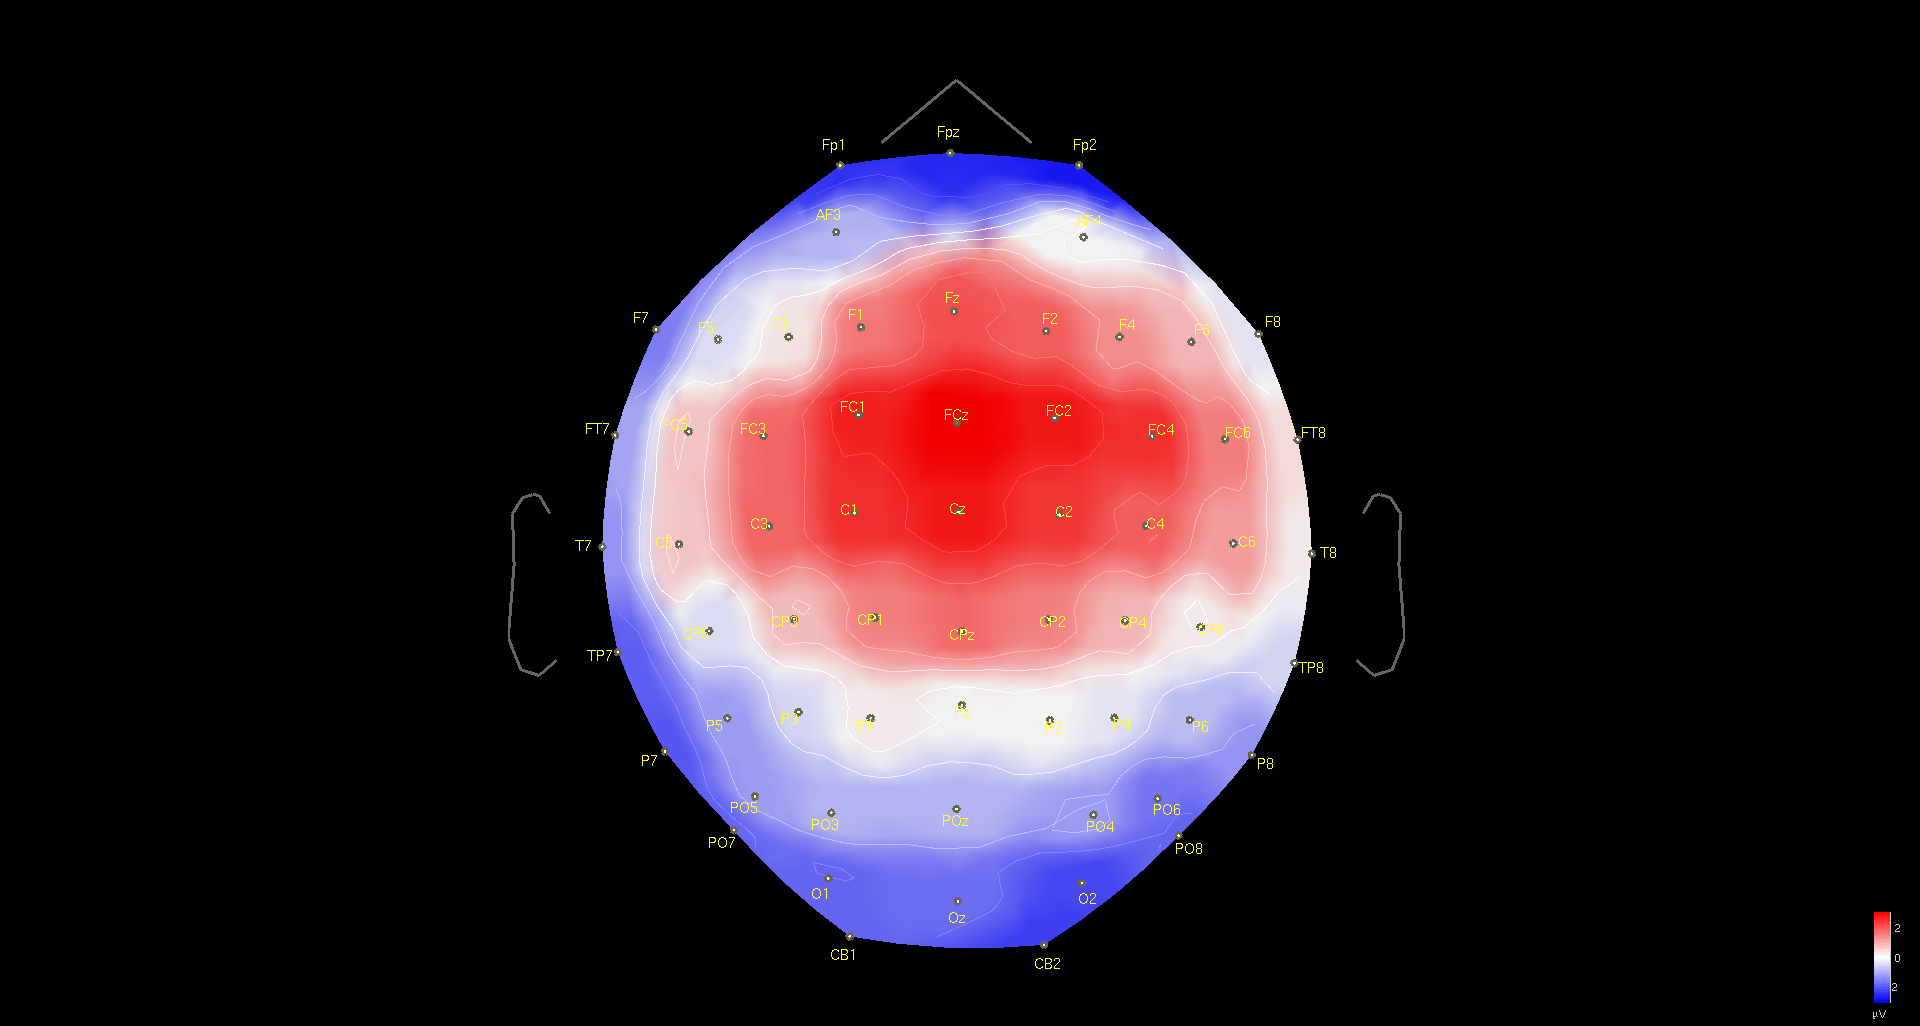
\includegraphics[width=3.5 in]{GA_Onset_P2_1000}
%\caption{Grand Average: Onset P2 1000 Hz}
%\label{fig:GA_Onset_P2_1000}
%\end{figure}
%%%%%%%%%%%% FIGURE (GA_Onset_P2_1000) %%%%%%%%%%%%
%
%%%%%%%%%%%% FIGURE (GA_Onset_P2_2000) %%%%%%%%%%%% 
%\begin{figure}[b]
%\centering
%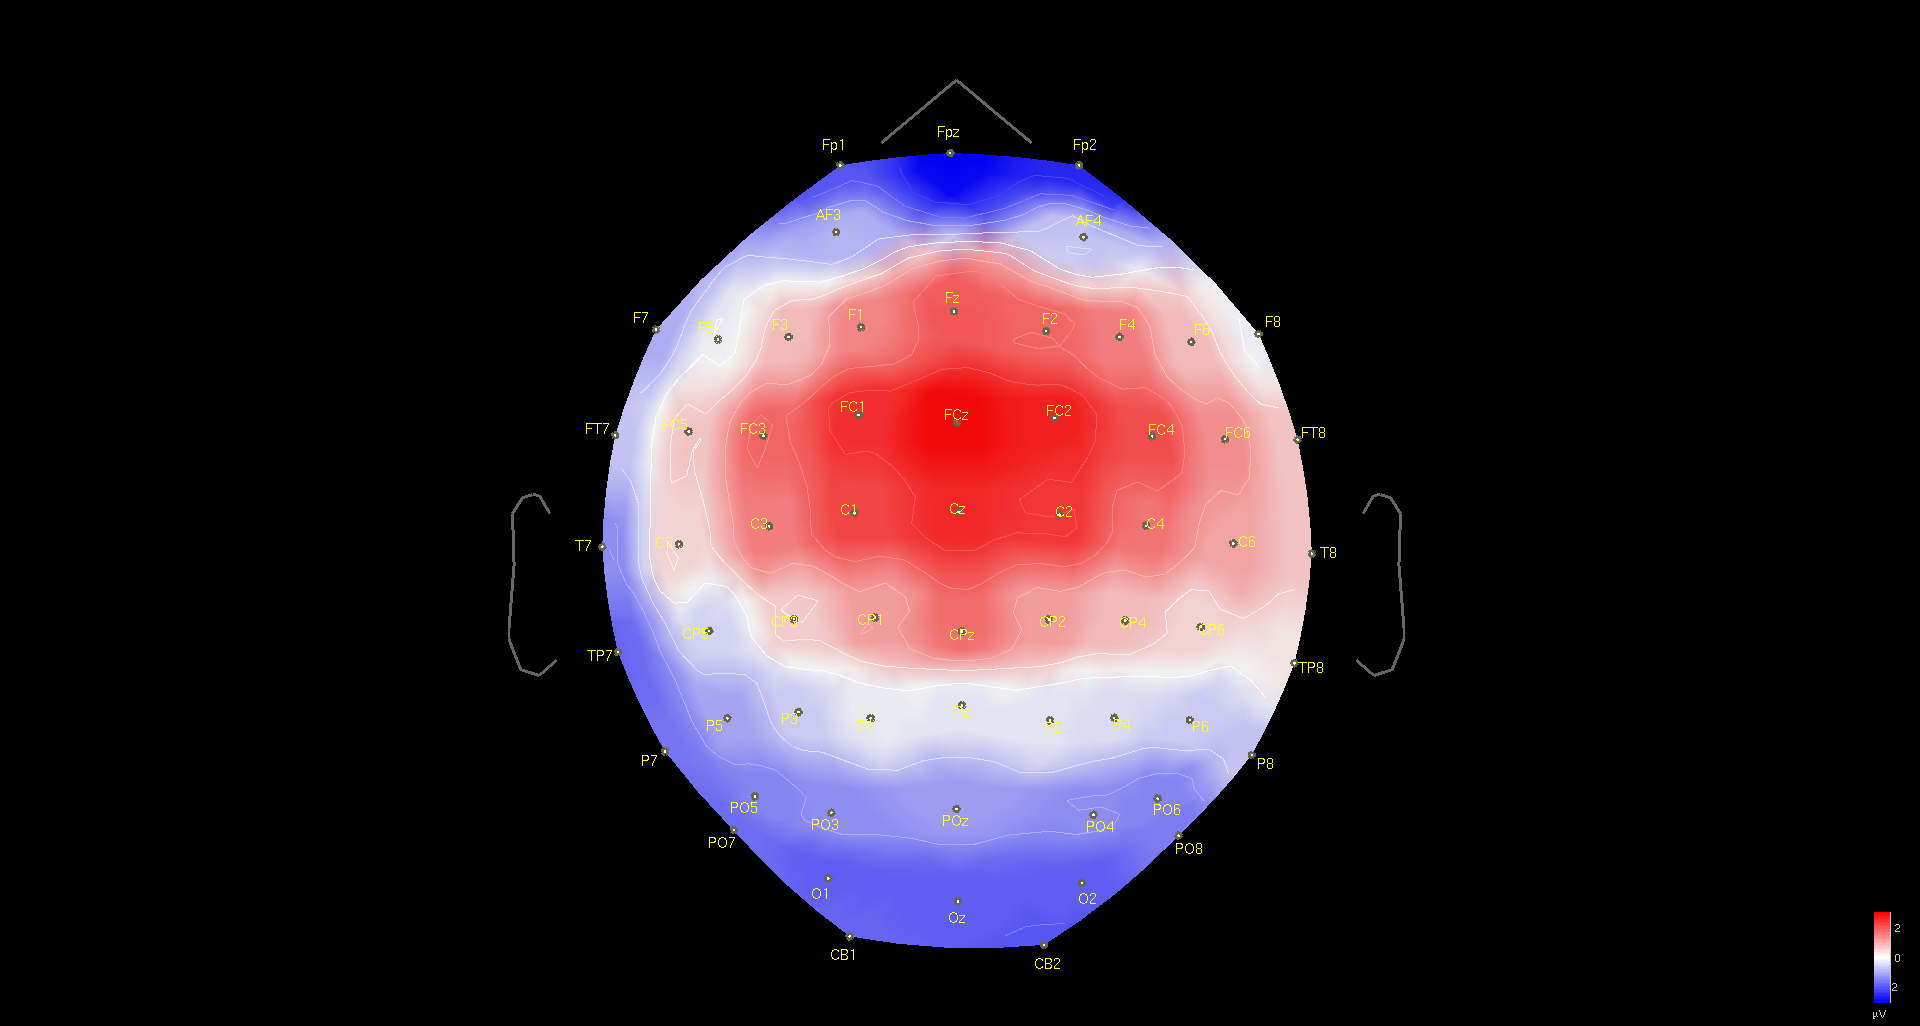
\includegraphics[width=3.5 in]{GA_Onset_P2_2000}
%\caption{Grand Average: Onset P2 2000 Hz}
%\label{fig:GA_Onset_P2_2000}
%\end{figure}
%%%%%%%%%%%% FIGURE (GA_Onset_P2_2000) %%%%%%%%%%%%
%
%%%%%%%%%%%% FIGURE (GA_Onset_P2_4000) %%%%%%%%%%%% 
%\begin{figure}[b]
%\centering
%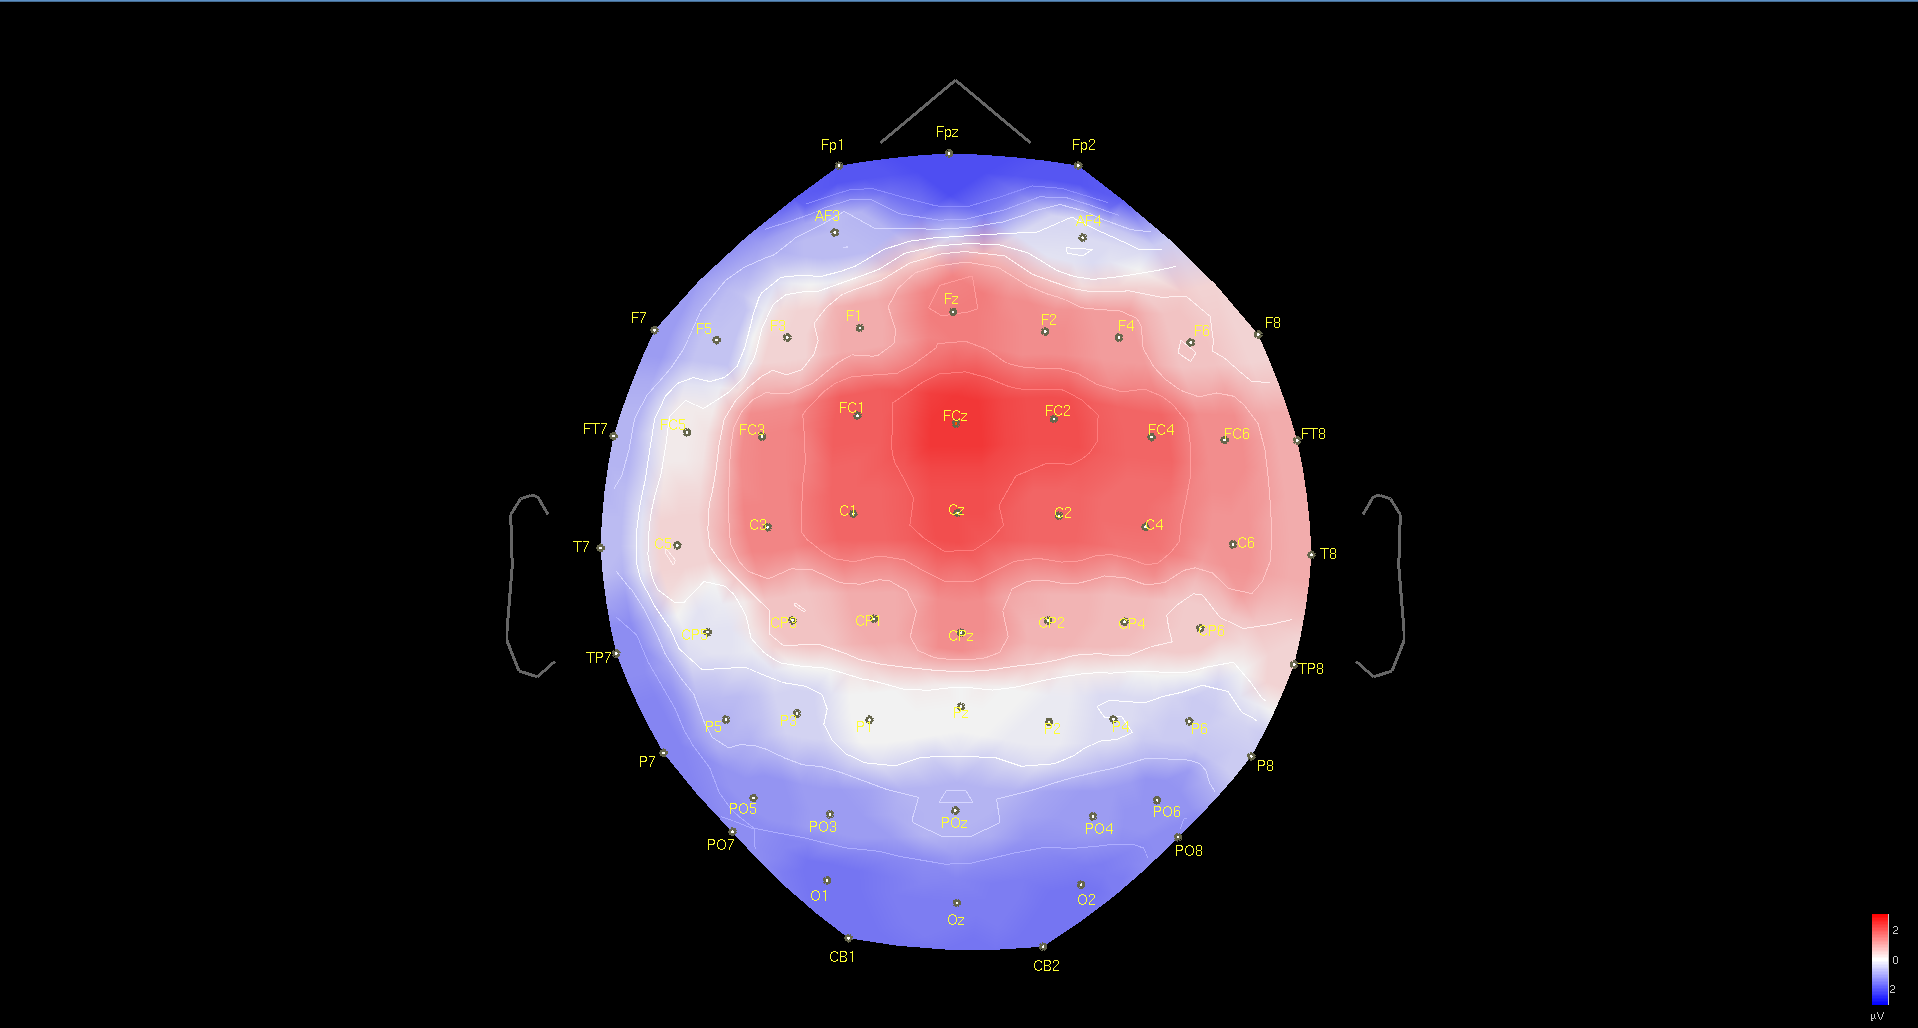
\includegraphics[width=3.5 in]{GA_Onset_P2_4000}
%\caption{Grand Average: Onset P2 4000 Hz}
%\label{fig:GA_Onset_P2_4000}
%\end{figure}
%%%%%%%%%%%% FIGURE (GA_Onset_P2_4000) %%%%%%%%%%%%
%
%
%
%\clearpage
%
%-------------------------------------------------------------------------------------------------
%	           CHANGE RESPONSE	           CHANGE RESPONSE
%-------------------------------------------------------------------------------------------------
%
%--------------------------------------
%	       CHANGE N1
%--------------------------------------
%
%%%%%%%%%%%% FIGURE (GA_Change_N1_500) %%%%%%%%%%%% 
%\begin{figure}[]
%\centering
%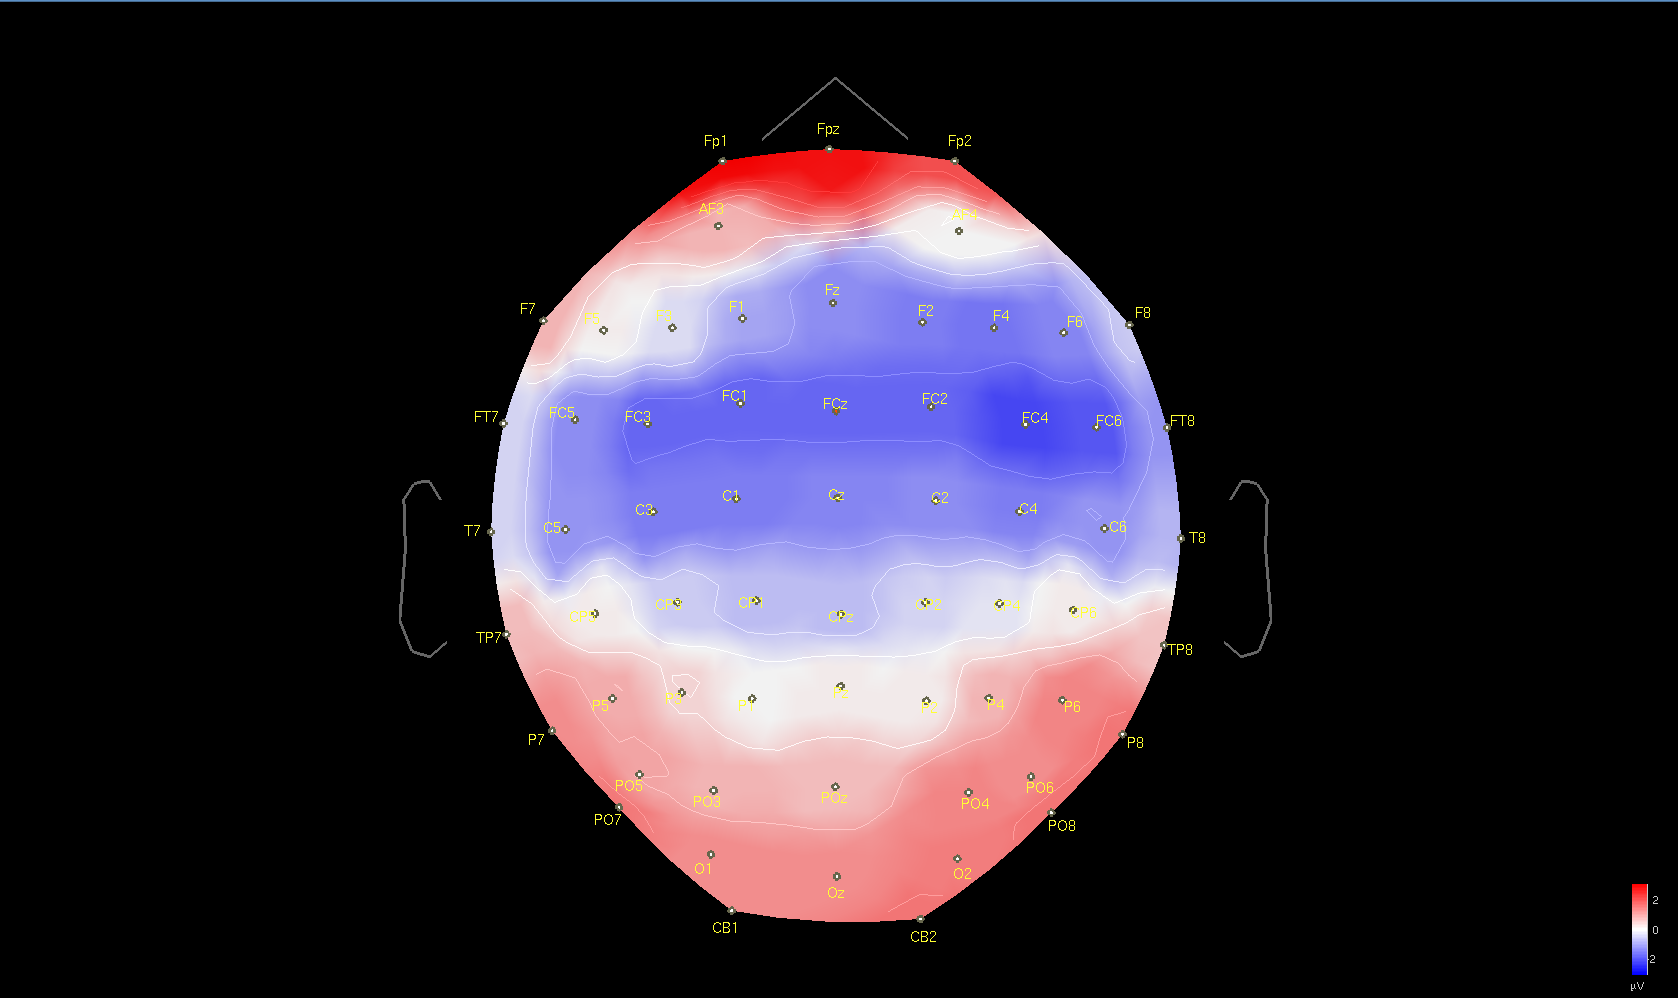
\includegraphics[width=3.5 in]{GA_Change_N1_500}
%\caption{Grand Average: Change N1 500 Hz}
%\label{fig:GA_Change_N1_500}
%\end{figure}
%%%%%%%%%%%% FIGURE (GA_Change_N1_500) %%%%%%%%%%%%
%
%%%%%%%%%%%% FIGURE (GA_Change_N1_1000) %%%%%%%%%%%% 
%\begin{figure}[]
%\centering
%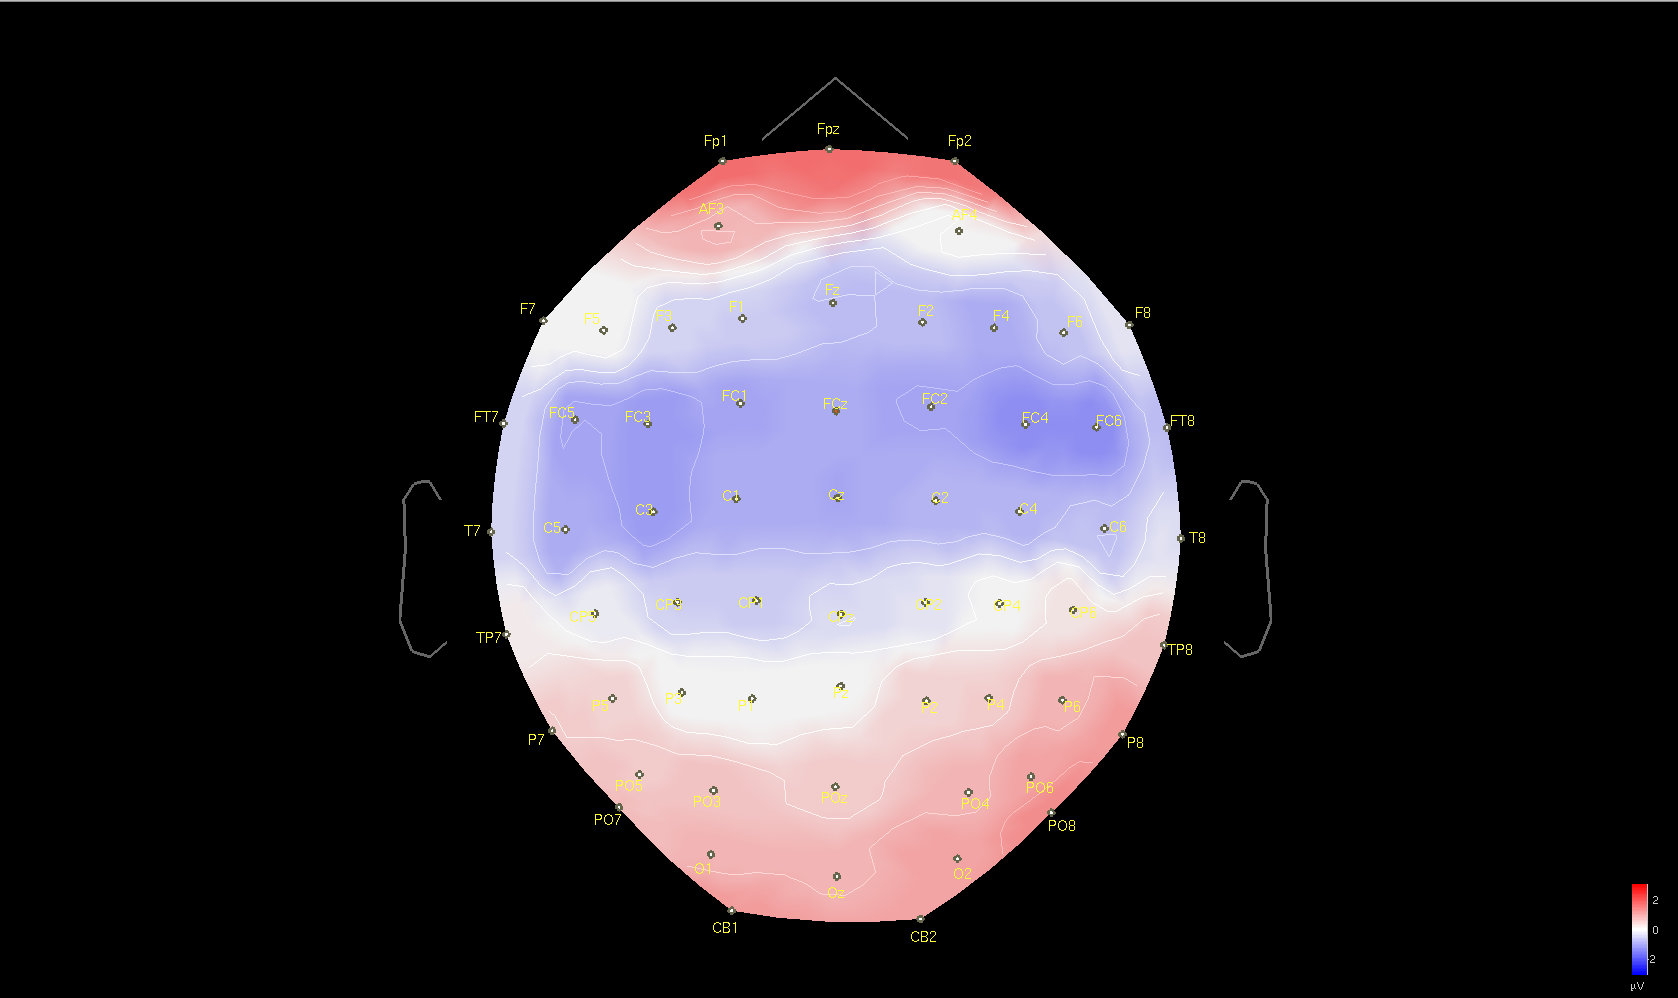
\includegraphics[width=3.5 in]{GA_Change_N1_1000}
%\caption{Grand Average: Change N1 1000 Hz}
%\label{fig:GA_Change_N1_1000}
%\end{figure}
%%%%%%%%%%%% FIGURE (GA_Change_N1_1000) %%%%%%%%%%%%
%
%%%%%%%%%%%% FIGURE (GA_Change_N1_2000) %%%%%%%%%%%% 
%\begin{figure}[]
%\centering
%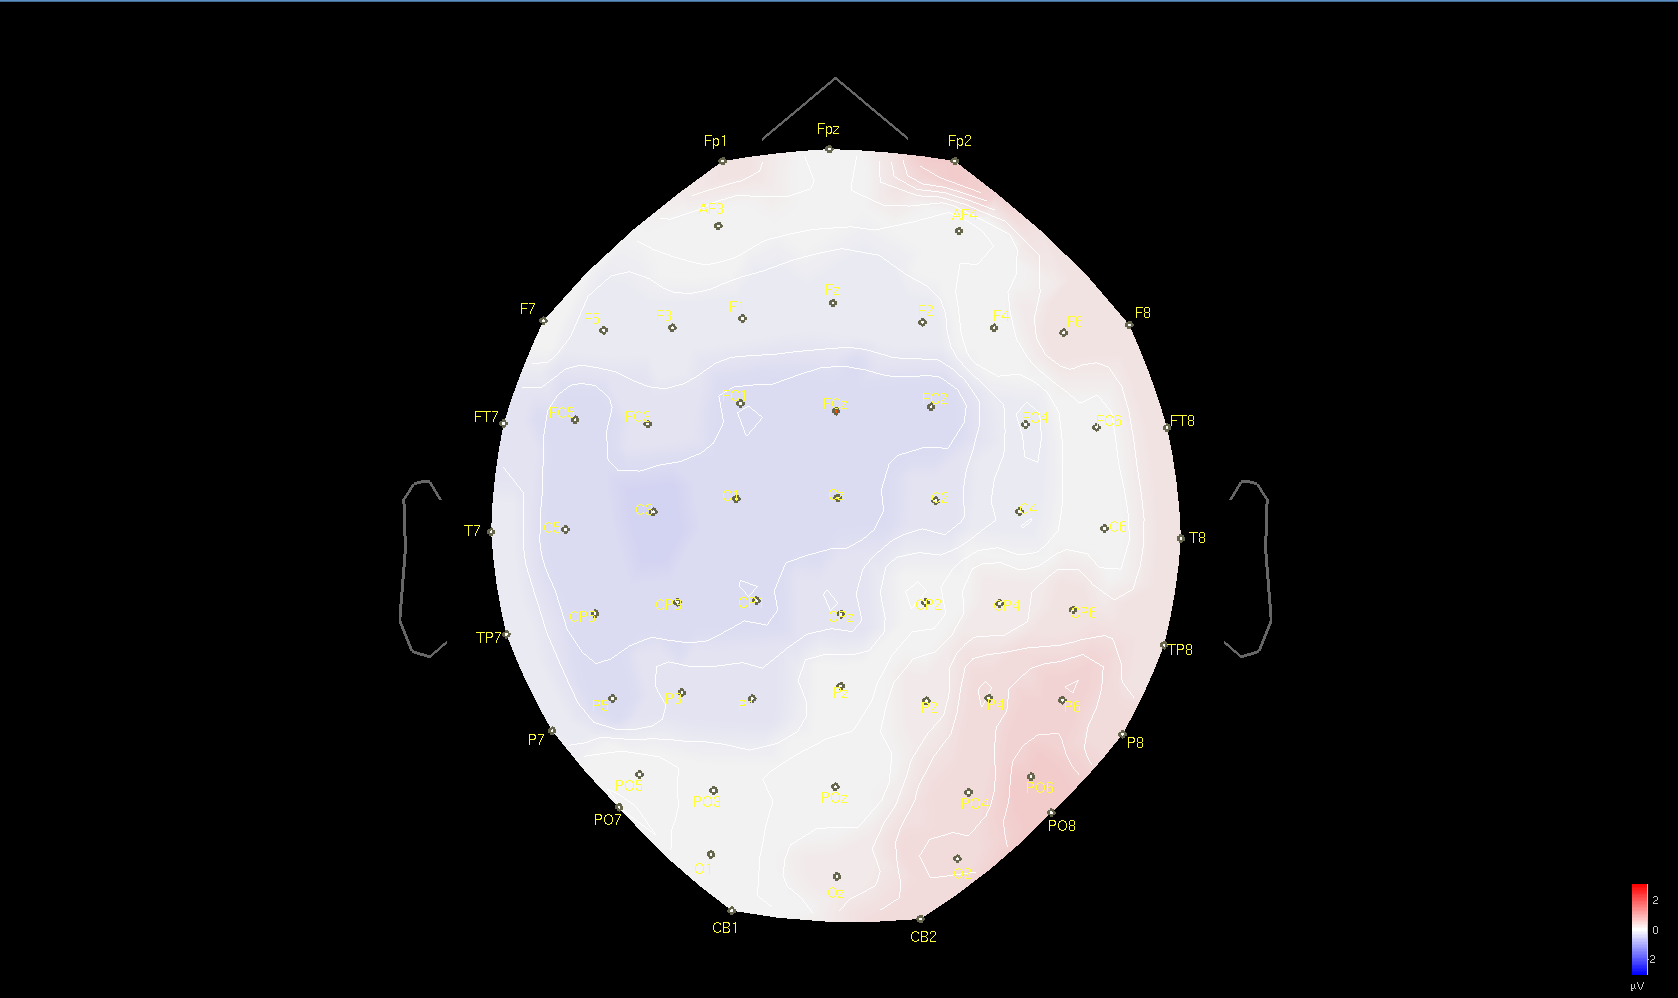
\includegraphics[width=3.5 in]{GA_Change_N1_2000}
%\caption{Grand Average: Change N1 2000 Hz}
%\label{fig:GA_Change_N1_2000}
%\end{figure}
%%%%%%%%%%%% FIGURE (GA_Change_N1_2000) %%%%%%%%%%%%
%
%
%%%%%%%%%%%% FIGURE (GA_Change_N1_4000) %%%%%%%%%%%% 
%\begin{figure}[]
%\centering
%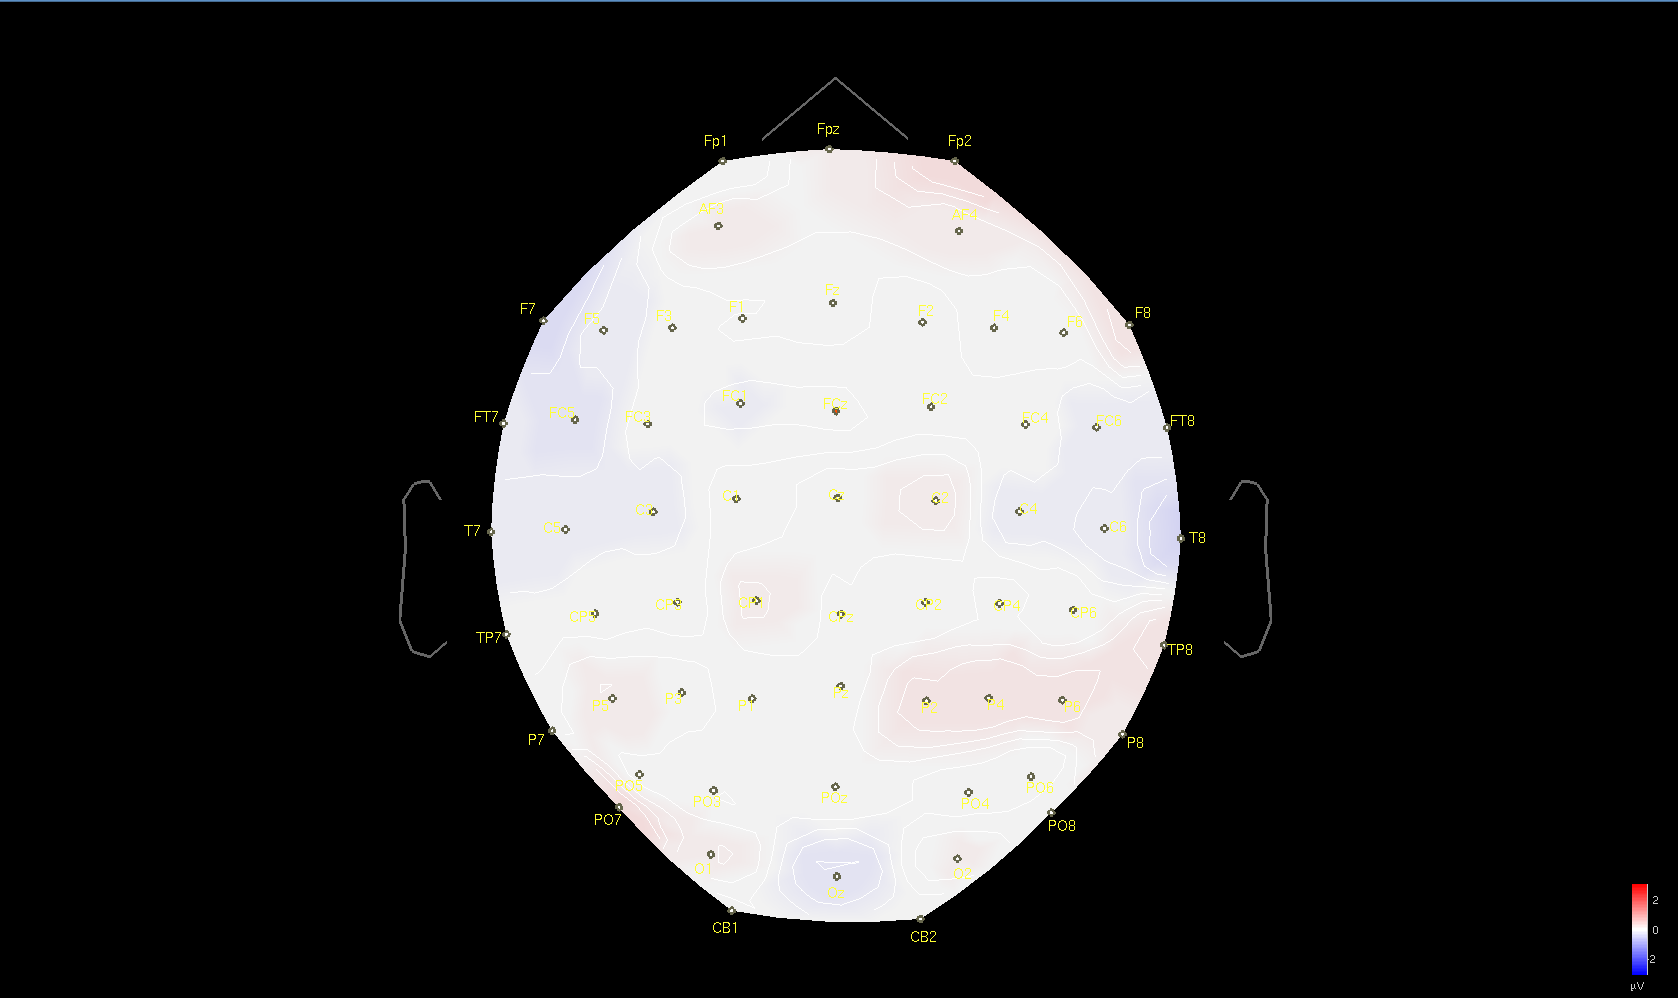
\includegraphics[width=3.5 in]{GA_Change_N1_4000}
%\caption{Grand Average: Change N1 4000 Hz}
%\label{fig:GA_Change_N1_4000}
%\end{figure}
%%%%%%%%%%%% FIGURE (GA_Change_N1_4000) %%%%%%%%%%%%
%
%--------------------------------------
%	       CHANGE P2
%--------------------------------------
%
%%%%%%%%%%%% FIGURE (GA_Change_P2_500) %%%%%%%%%%%% 
%\begin{figure}[]
%\centering
%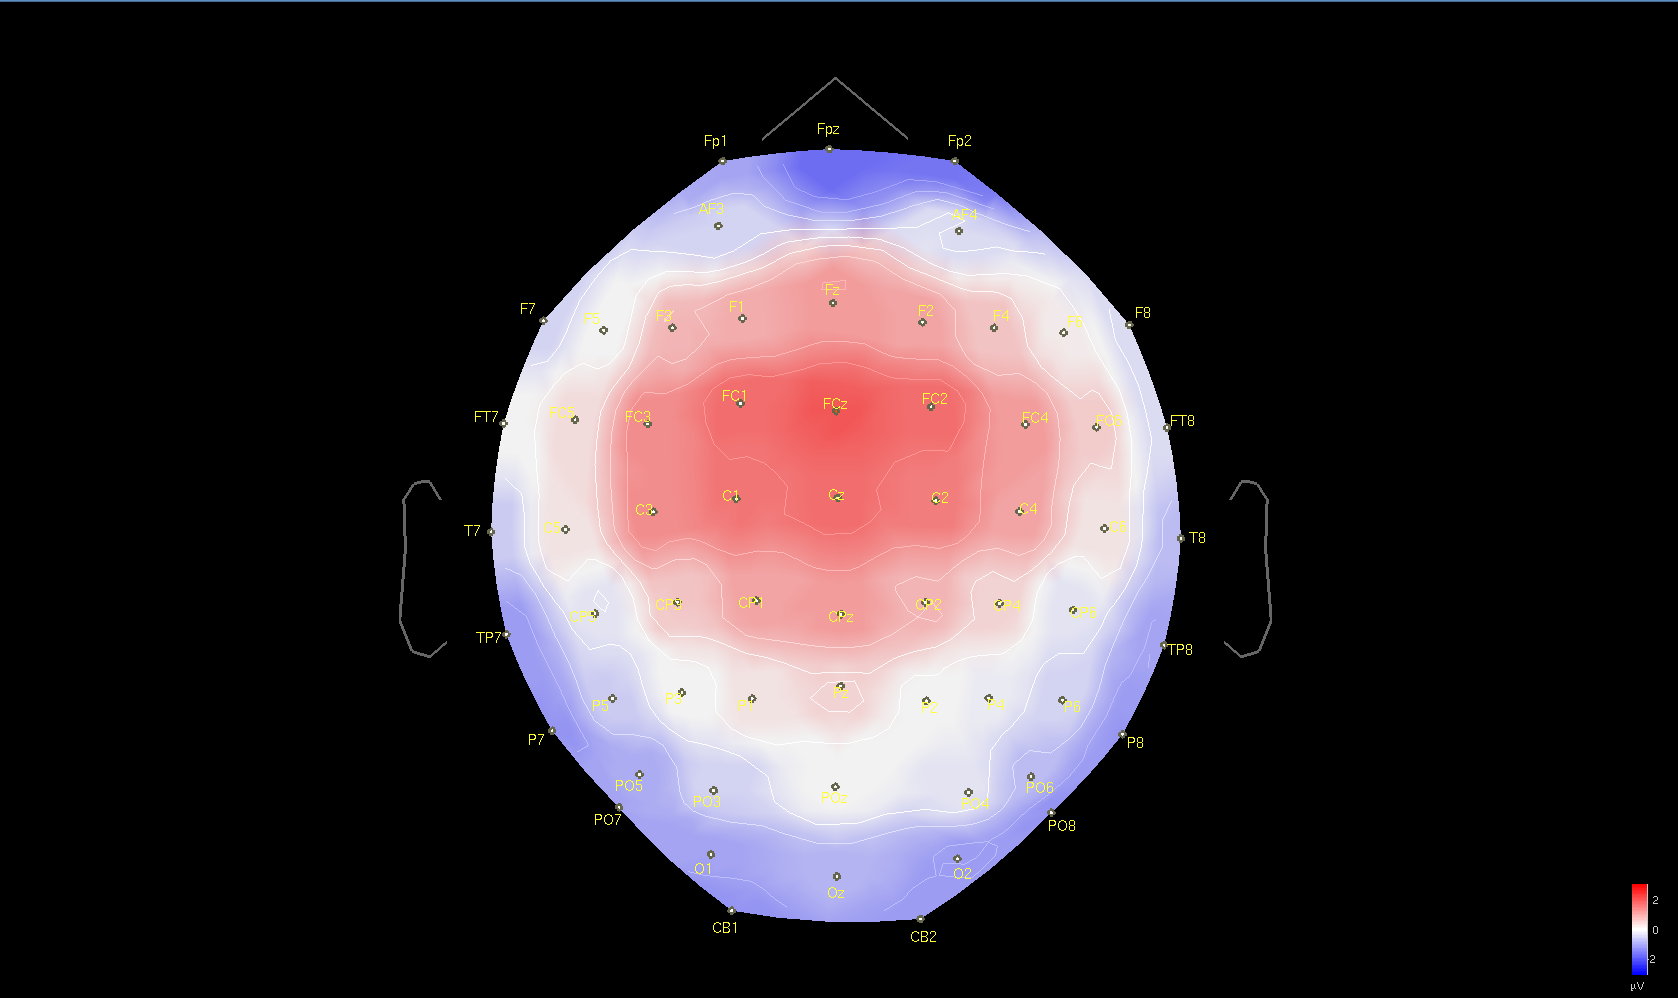
\includegraphics[width=3.5 in]{GA_Change_P2_500}
%\caption{Grand Average: Change P2 500 Hz}
%\label{fig:GA_Change_P2_500}
%\end{figure}
%%%%%%%%%%%% FIGURE (GA_Change_P2_500) %%%%%%%%%%%%
%
%%%%%%%%%%%% FIGURE (GA_Change_P2_1000) %%%%%%%%%%%% 
%\begin{figure}[]
%\centering
%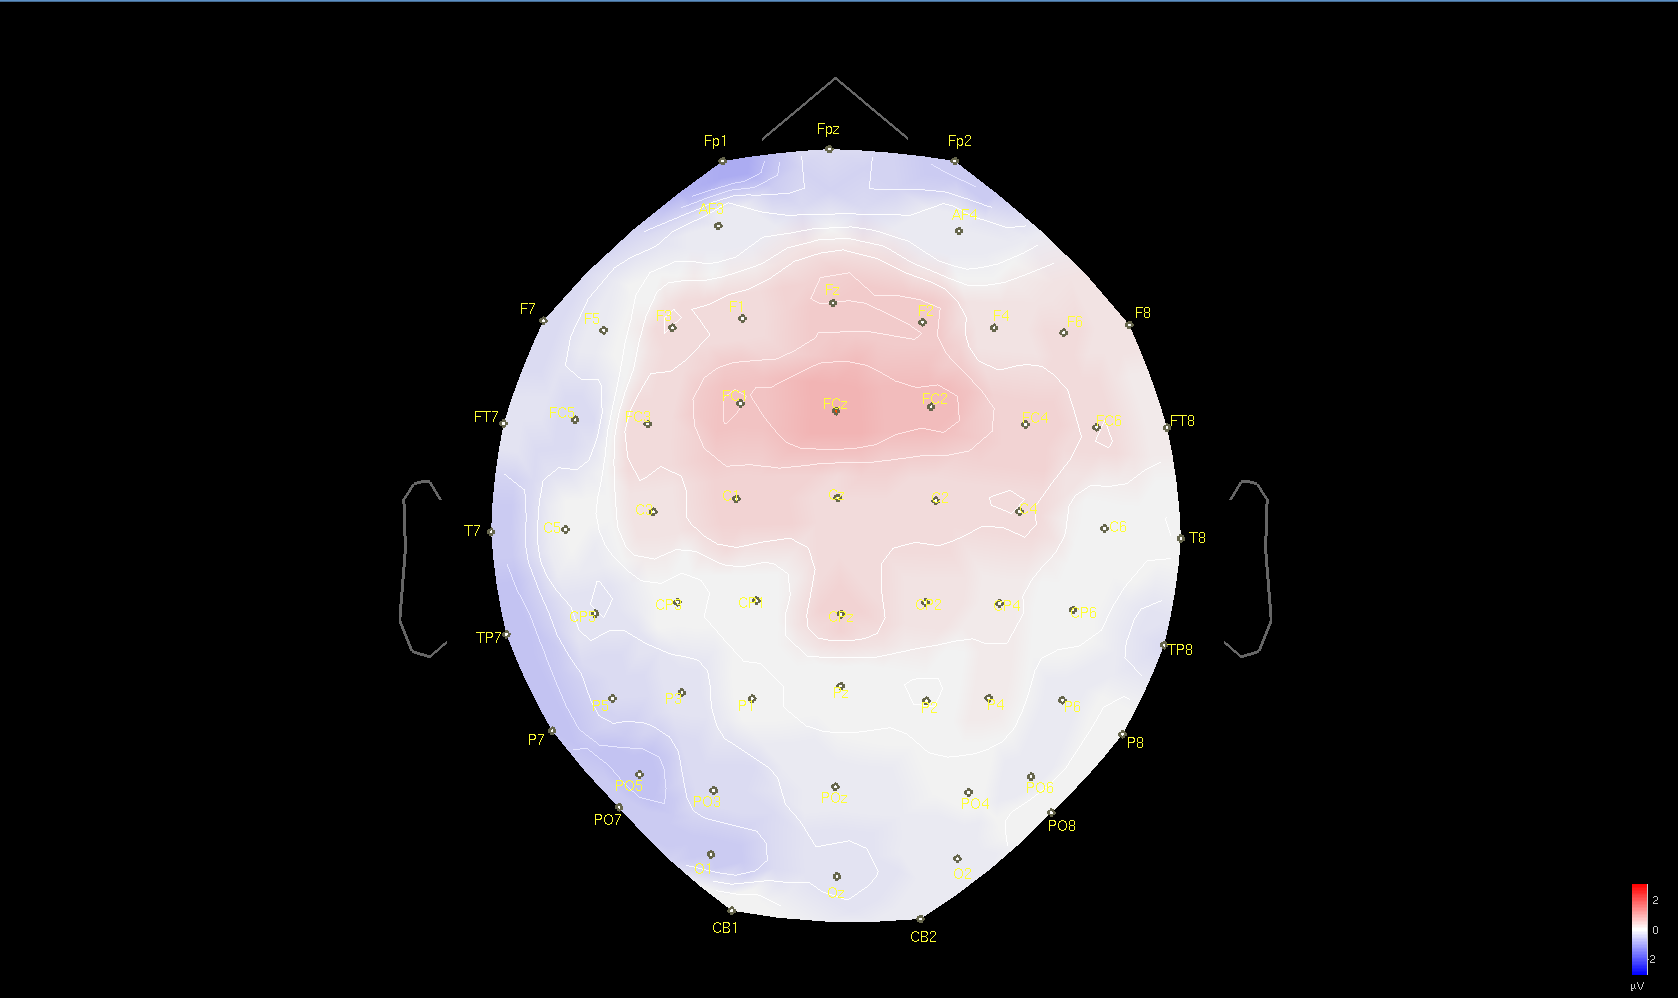
\includegraphics[width=3.5 in]{GA_Change_P2_1000}
%\caption{Grand Average: Change P2 1000 Hz}
%\label{fig:GA_Change_P2_1000}
%\end{figure}
%%%%%%%%%%%% FIGURE (GA_Change_P2_1000) %%%%%%%%%%%%
%
%%%%%%%%%%%% FIGURE (GA_Change_P2_2000) %%%%%%%%%%%% 
%\begin{figure}[b]
%\centering
%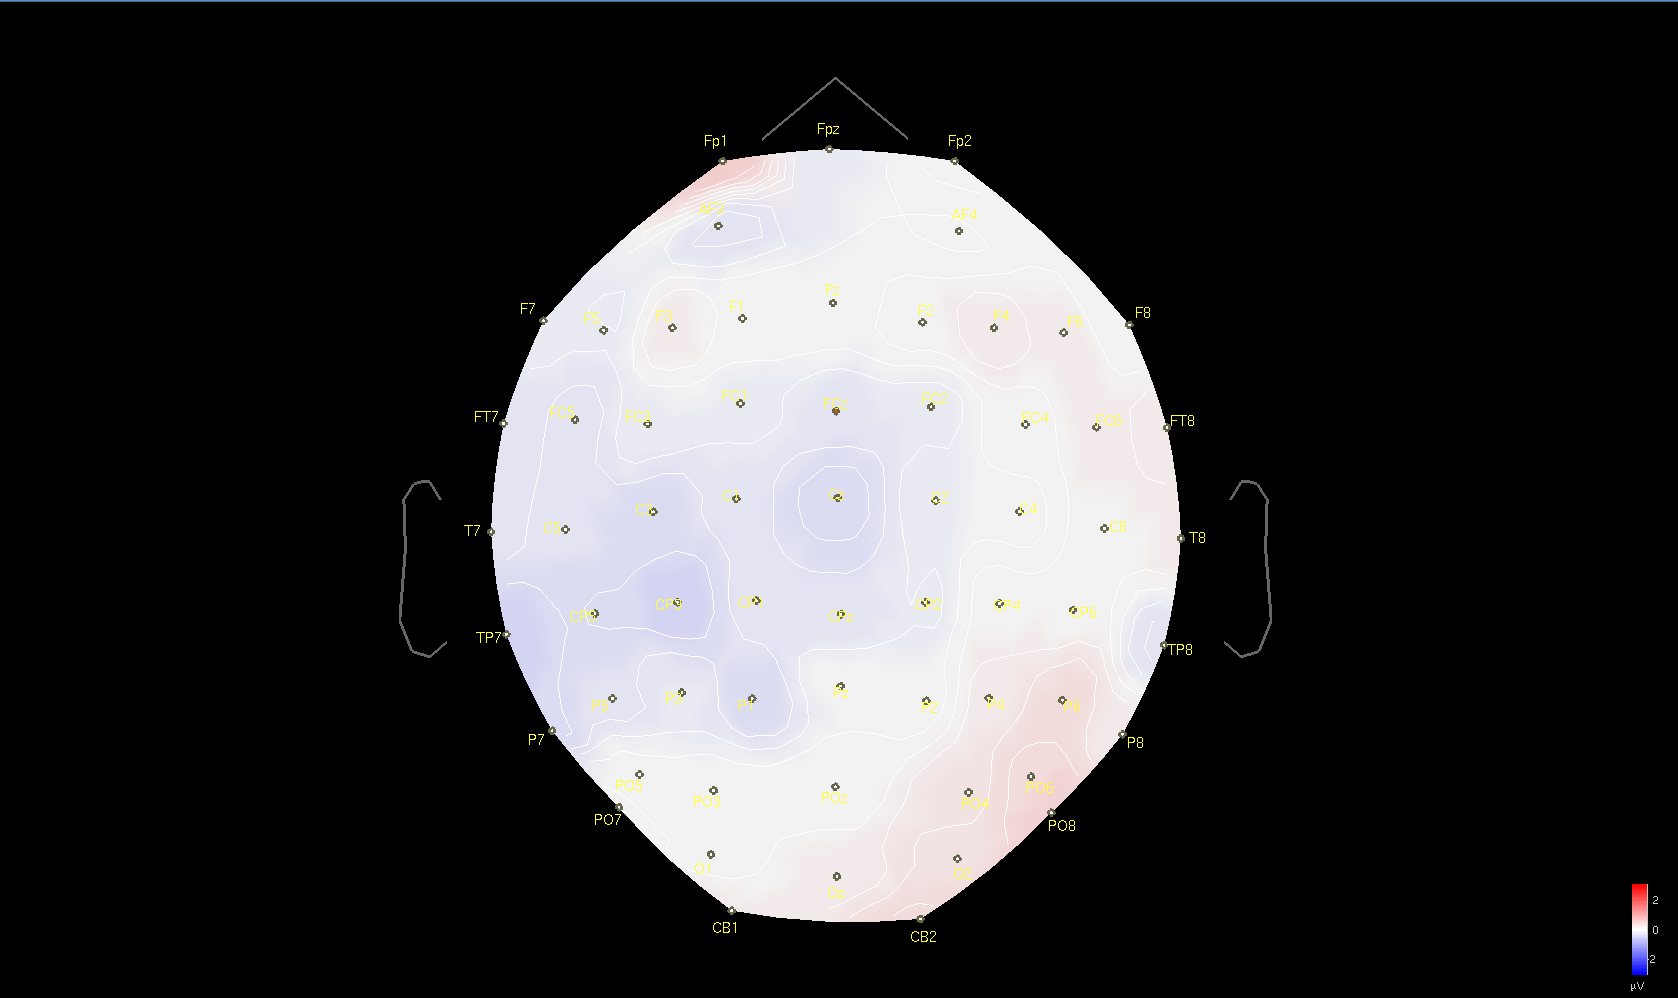
\includegraphics[width=3.5 in]{GA_Change_P2_2000}
%\caption{Grand Average: Change P2 2000 Hz}
%\label{fig:GA_Change_P2_2000}
%\end{figure}
%%%%%%%%%%%% FIGURE (GA_Change_P2_2000) %%%%%%%%%%%%
%
%
%%%%%%%%%%%% FIGURE (GA_Change_P2_4000) %%%%%%%%%%%% 
%\begin{figure}[b]
%\centering
%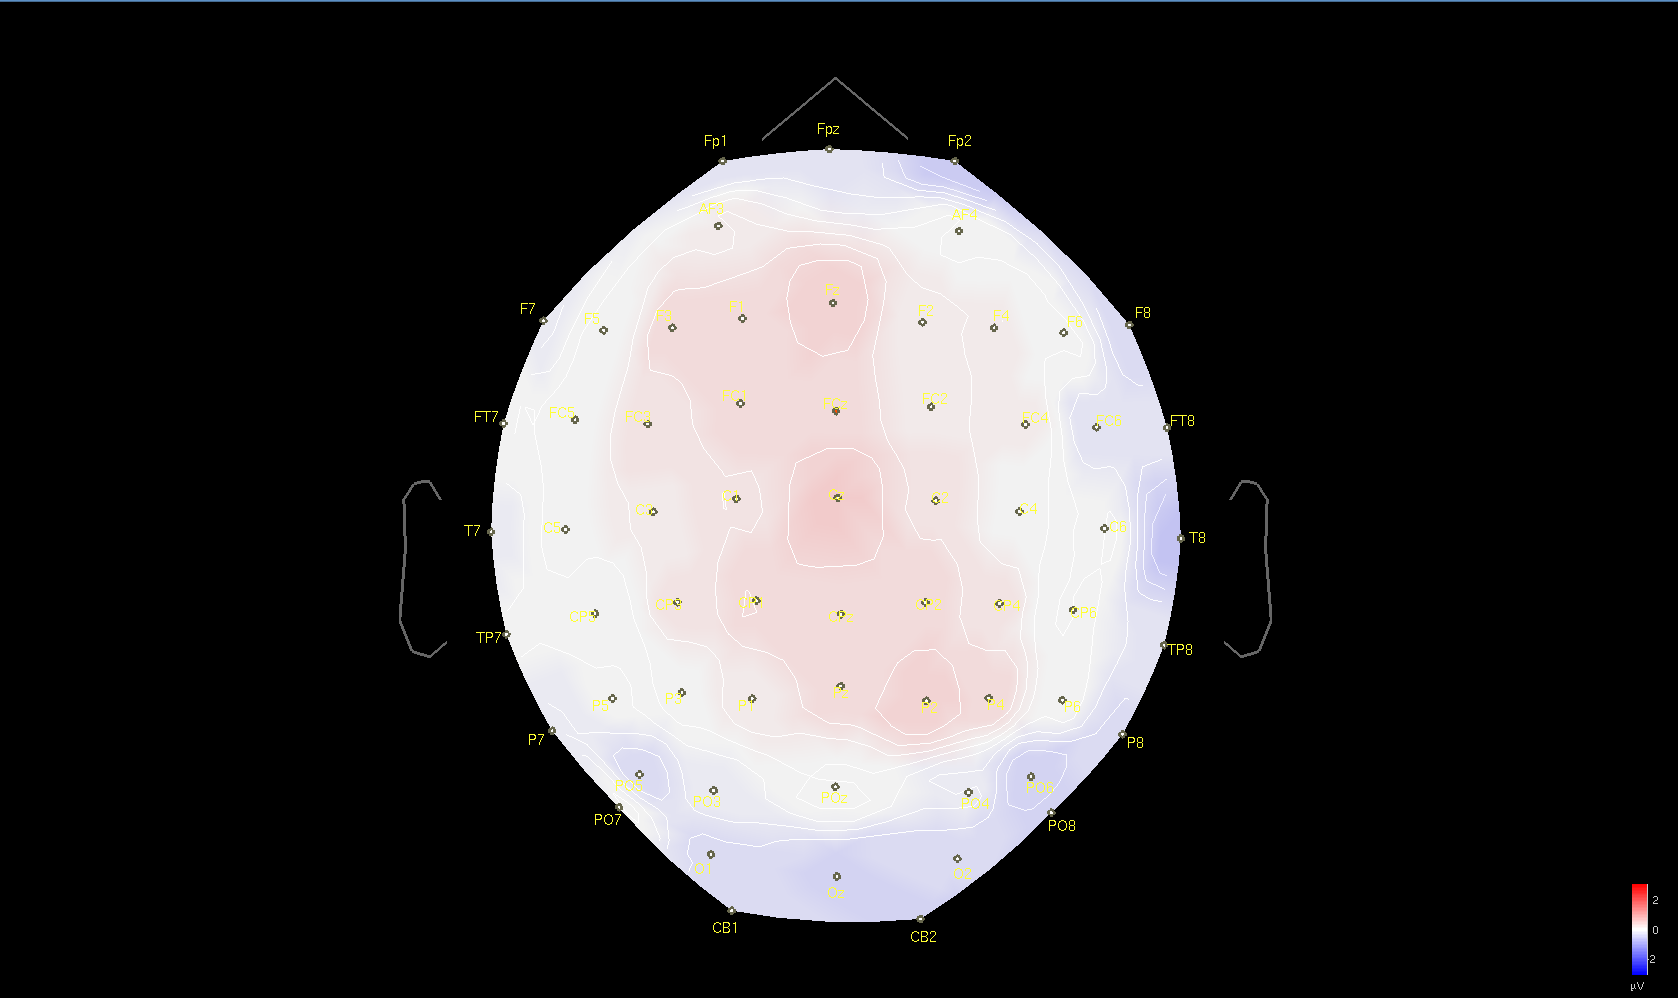
\includegraphics[width=3.5 in]{GA_Change_P2_4000}
%\caption{Grand Average: Change P2 4000 Hz}
%\label{fig:GA_Change_P2_4000}
%\end{figure}
%%%%%%%%%%%% FIGURE (GA_Change_P2_4000) %%%%%%%%%%%%

\end{document}
